%
% Modelo de trabalho acadêmico (Teses, Dissertações, TCC)
% Documento principal
%
% Centro Federal de Educação Tecnológica de Minas Gerais - CEFET-MG
% Autor: Cristiano Fraga G. Nunes <cfgnunes@gmail.com>
%
% Projeto hospedado em: https://github.com/cfgnunes/latex-cefet-mg
%
%
% Informações:
%   Codificação utilizada: UTF-8
%   Tamanho da tabulação: 4 (espaços)


\documentclass[oneside]{abntex2-cefetmg}            % Imprimir apenas frente
%\documentclass[doubleside]{abntex2-cefetmg}        % Imprimir frente e verso

% Importações de pacotes
\usepackage[portuguese, onelanguage, lined, boxed, commentsnumbered, algoruled]{algorithm2e}                % Escrever algoritmos
\usepackage[alf, abnt-emphasize=bf, bibjustif, recuo=0cm, abnt-etal-cite=2, abnt-etal-list=0]{abntex2cite}  % Citações padrão ABNT
\usepackage[utf8]{inputenc}                         % Acentuação direta
\usepackage[T1]{fontenc}                            % Codificação da fonte em 8 bits
\usepackage{graphicx}                               % Inserir figuras
\usepackage{amsfonts, amssymb, amsmath}             % Fonte e símbolos matemáticos
\usepackage{booktabs}                               % Comandos para tabelas
\usepackage{verbatim}                               % Texto é interpretado como escrito no documento
\usepackage{multirow, array}                        % Múltiplas linhas e colunas em tabelas
\usepackage{indentfirst}                            % Endenta o primeiro parágrafo de cada seção.
\usepackage{microtype}                              % Para melhorias de justificação?
\usepackage{float}                                  % Utilizado para criação de floats
\usepackage{icomma}                                 % Uso de vírgulas em expressões matemáticas
\usepackage{palatino}                               % Usa a fonte Palatino
%\usepackage{times}                                 % Usa a fonte Times
%\usepackage{lmodern}                               % Usa a fonte Latin Modern
%\usepackage{color, colortbl}                       % Comandos de cores
\usepackage[table,xcdraw]{xcolor}                   % Comandos de cores hexadecimais
\usepackage{listings}                              % Importação de códigos fonte
\usepackage[bottom]{footmisc}                      % Mantém as notas de rodapé sempre na mesma posição
%\usepackage{subfig}                                % Posicionamento de figuras
%\usepackage{scalefnt}                              % Permite redimensionar tamanho da fonte
%\usepackage{lscape}                                % Permite páginas em modo "paisagem"
%\usepackage{picinpar}                              % Dispor imagens em parágrafos
\usepackage{ltablex}

% Inclui o preâmbulo do documento
%
% Documento: Preâmbulo
%

\titulo{Otimizando Desempenho de \textit{Front-end} em \textit{Websites} para HTTP2}
%\title{Optimizing Websites' Front-end Performance for HTTP2}
%\subtitulo{Subtítulo do trabalho}
\autor{Pedro Colen Cardoso}
\local{Belo Horizonte}
\data{Julho de 2015}
\instituicao{Centro Federal de Educação Tecnológica de Minas Gerais}
\departamento{Departamento de Computação}
\programa{Curso de Engenharia de Computação}
\tipotrabalho{Monografia}
\preambulo{Trabalho de Conclusão de Curso apresentado ao Curso de Engenharia da Computação do Centro Federal de Educação Tecnológica de Minas Gerais.}
\orientador{Flávio Roberto dos Santos Coutinho}
%\orientador[Orientadora:]{Nome da orientadora}
\titulacaoOrientador{Prof. }
\instOrientador{Centro Federal de Educação Tecnológica de Minas Gerais -- CEFET-MG}
%\coorientador{Nome do coorientador}
%\coorientador[Coorientadora:]{Nome da coorientadora}
%\titulacaoCoorientador{Prof. Dr. }
%\instCoorientador{Centro Federal de Educação Tecnológica de Minas Gerais -- CEFET-MG}
%\areaconcentracao{Modelagem Matemática e Computacional}
%\linhapesquisa{Sistemas Inteligentes}


% Define as cores dos links e informações do PDF
\makeatletter
\hypersetup{
    portuguese,
    colorlinks,
    linkcolor=blue,
    citecolor=blue,
    filecolor=blue,
    urlcolor=blue,
    breaklinks=true,
    pdftitle={\@title},
    pdfauthor={\@author},
    pdfsubject={\imprimirpreambulo},
    pdfkeywords={abnt, latex, abntex, abntex2}
}
\makeatother

% Redefinição de labels
\renewcommand{\algorithmautorefname}{Algoritmo}
\def\equationautorefname~#1\null{Equa\c c\~ao~(#1)\null}

% Cria o índice remissivo
\makeindex

% Início do documento
\begin{document}

    % Retira espaço extra obsoleto entre as frases
    \frenchspacing

    % Elementos pré textuais
    \pretextual
    %
% Documento: Capa
%

\makeatletter
\begin{capa}

    \hspace{-2.0cm}
    \begin{minipage}{0.19\textwidth}
        
\includegraphics[width=0.8\textwidth]{./04-figuras/cefet-logo}
    \end{minipage}
    \quad
    \hspace{-1.5cm}
    \begin{minipage}{.9\textwidth}
        \begin{center}
        \normalfont\scshape{\imprimirinstituicao}\\
        \normalfont\scshape{\imprimirdepartamento}\\
        \normalfont\scshape{\imprimirprograma}\\
        \abntex@ifnotempty{\imprimirareaconcentracao}
        {%
            \normalfont\scshape{\imprimirareaconcentracao}
        }
        \end{center}
    \end{minipage}

    \vspace*{200pt}

    \begin{center}
        \ABNTEXchapterfont\Large\scshape\imprimirtitulo
        \abntex@ifnotempty{\imprimirsubtitulo}{%
            {\ABNTEXchapterfont\Large\scshape: }{\ABNTEXchapterfont\large\scshape\imprimirsubtitulo}
        }
    \end{center}

    \vspace*{80pt}

    \begin{center}
        \large\normalfont\scshape\textbf\imprimirautor
    \end{center}

    \vspace*{10pt}

    \begin{center}
        \small\imprimirorientadorRotulo{} \imprimirTitulacaoOrientador \imprimirorientador \\
        \small\imprimirinstOrientador \\
        \abntex@ifnotempty{\imprimircoorientador}
        {%
            \begin{SingleSpacing}\par\end{SingleSpacing}
            \small\imprimircoorientadorRotulo{} \imprimirTitulacaoCoorientador \imprimircoorientador \\
            \small\imprimirinstCoorientador
        }
    \end{center}

    \vspace*{\fill}

    \begin{center}
        \normalfont\scshape{\imprimirlocal}\\
        \normalfont\scshape{\imprimirdata}
    \end{center}

\end{capa}
\makeatother
              % Capa
    %
% Documento: Folha de rosto
%

\makeatletter
\begin{folhaderosto}

    \begin{center}
        {\large\normalfont\scshape\textbf\imprimirautor}
    \end{center}

    \vspace*{150pt}

    \begin{center}
        \ABNTEXchapterfont\Large\scshape\imprimirtitulo
        \abntex@ifnotempty{\imprimirsubtitulo}{%
            {\ABNTEXchapterfont\Large\scshape: }{\ABNTEXchapterfont\large\scshape\imprimirsubtitulo}
        }
    \end{center}

    \vspace*{90pt}

    \abntex@ifnotempty{\imprimirpreambulo}{%
        \SingleSpacing
        \begin{tabular}{p{.24\textwidth}p{.15\textwidth}p{.44\textwidth}}
            & \multicolumn{2}{p{.6\textwidth}}{\small\hyphenpenalty=10000{\imprimirpreambulo}} \\ & & \\
            \abntex@ifnotempty{\imprimirareaconcentracao}
            {%
                & \multicolumn{2}{p{.6\textwidth}}{\small\hyphenpenalty=10000{\imprimirareaconcentracaoRotulo\imprimirareaconcentracao}} \\ & & \\
            }
            \abntex@ifnotempty{\imprimirlinhapesquisa}
            {%
                & \multicolumn{2}{p{.6\textwidth}}{\small\hyphenpenalty=10000{\imprimirlinhapesquisaRotulo\imprimirlinhapesquisa}} \\ & & \\
            }
            & \small\imprimirorientadorRotulo & \imprimirorientador \\
            & & \small\imprimirinstOrientador \\ & & \\
            \abntex@ifnotempty{\imprimircoorientador}
            {%
                & \small\imprimircoorientadorRotulo & \imprimircoorientador \\
                & & \small\imprimirinstCoorientador
            }
        \end{tabular}
    }

    \vspace*{\fill}

    \begin{center}
        \normalfont\scshape{\imprimirinstituicao}\\
        \normalfont\scshape{\imprimirdepartamento}\\
        \normalfont\scshape{\imprimirprograma}\\
        \normalfont\scshape{\imprimirlocal}\\
        \normalfont\scshape{\imprimirdata}
    \end{center}

\end{folhaderosto}
\makeatother
       % Folha de rosto
    %%
% Documento: Folha de aprovação
%



%
% Documento: Folha de aprovação
%

\makeatletter
\begin{folhadeaprovacao}
		\hspace{-2.0cm}
	    \begin{minipage}{0.19\textwidth}
	    	
\includegraphics[width=0.8\textwidth]{./04-figuras/cefet-logo}
	    \end{minipage}
	    \quad
	    \hspace{-1.5cm}
	    \begin{minipage}{.9\textwidth}
	    	\begin{center}	    	
	    	{\normalfont\scshape\textbf\imprimirinstituicao}\\
	    	\normalfont\scshape{\imprimirdepartamento}\\
	    	\normalfont\scshape{\imprimirprograma}\\
	    	{\normalfont\scshape Avalia\c{c}\~ao do Trabalho de Conclusão de Curso}\\
	    	\end{center}
	    \end{minipage}
	
	\vspace*{50pt}
	
	{\noindent\normalfont\scshape\textbf{Aluno:} \imprimirautor}\\
	{\normalfont\scshape\textbf{T\'{i}tulo do trabalho:} \imprimirtitulo}\\
	{\normalfont\scshape\textbf{Data do trabalho:} 20/11/2015}\\
	{\normalfont\scshape\textbf{Hor\'{a}rio:} 16:00}\\
	{\normalfont\scshape\textbf{Local da defesa: Audit{\'o}rio 401, pr{\'e}dio 17 (DECOM).} }\\
	
	\vspace*{40pt}
	
	\begin{center}
		{\normalfont\scshape O presente Trabalho de Conclus\~ao de Curso foi avaliado pela seguinte banca:}\\
	\end{center}
	
	\vspace*{10pt}
	
	\begin{center}
		{\normalfont\scshape\imprimirorientador - Orientador}\\
		{\normalfont\scshape Departamento de Computa\c{c}\~ao}\\
		{\normalfont\scshape\imprimirinstituicao}\\
	\end{center}
	
	\vspace*{3pt}
	
	\begin{center}
		{\normalfont\scshape Profª. Glívia Angélica Rodrigues Barbosa - Membro da banca de avalia\c{c}\~ao}\\
		{\normalfont\scshape Departamento de Computa\c{c}\~ao}\\
		{\normalfont\scshape\imprimirinstituicao}\\
	\end{center}
	
	\vspace*{3pt}
	
	\begin{center}
		{\normalfont\scshape Prof. Ismael Santana Silva - Membro da banca de avalia\c{c}\~ao}\\
		{\normalfont\scshape Departamento de Computa\c{c}\~ao}\\
		{\normalfont\scshape\imprimirinstituicao}\\
	\end{center}
	
\end{folhadeaprovacao}
\makeatother
   % Folha de aprovação
    %%
% Documento: Dedicatória
%

\begin{dedicatoria}

Espaço reservado para dedicatória.
Inserir seu texto aqui...

\end{dedicatoria}
       % Dedicatória
    %%
% Documento: Agradecimentos
%

\begin{agradecimentos}

Gostaria de dedicar um agradecimento especial ao meu professor orientador, M.Sc. Flávio Roberto dos Santos Coutinho, produzir esse trabalho não foi fácil e ele esteve comigo durante toda a jornada. Também gostaria de agradecer à todos os professor do CEFET-MG que durante esse tempo me ensinaram a importância de se dedicar ao que amamos e que, apesar de todas as diversidades, sempre existe uma maneira de fazer as coisas acontecerem. Por fim quero agradecer minha família e meus amigos, pois sem eles nada disso faria sentido.

\end{agradecimentos}
    % Agradecimentos
    %
% Documento: Epígrafe
%

\begin{epigrafe}

\textit{``O fator decisivo para vencer o maior obstáculo é, invariavelmente, ultrapassar o obstáculo anterior.'' (Henry Ford)}
(esta página é opcional)

\end{epigrafe}
          % Epígrafe
    %
% Documento: Resumo (Português)
%

\begin{resumo}



\end{resumo}
         % Resumo na língua vernácula
    %
% Documento: Resumo (Inglês)
%

\begin{resumo}[Abstract]

Since the 90s the Web has not stoped expanding and acquiring new features. Nowadays the most popular part of the Internet is not made of static pages used just for reading. Along with the evolution of the Web, the amount of data exchanged between servers and final users has increased considerably, and that is because of the complexity of the web pages. An increase in pages' load time results in dissatisfied users and financial losses for companies. To reduce this wait time, Steve Souders dedicated his career to find techniques to optimize the performance of the front-end of websites. His techniques have been proved efficient for HTTP/1.1, that was the ruling version of the protocol for a long day. With the imminent release of HTTP/2, the techniques created by Souders might not work in the new protocol. This work analyzed the techniques proposed by Steve Souders, found the ones that could be affected by the changes in the HTTP protocol and tested them in the new version. The result obtained in this work is a list of techniques for front-end performance optimization that work in the protocol HTTP/2. 

\end{resumo}
         % Resumo em língua estrangeira
    %
% Documento: Lista de figuras
%

\pdfbookmark[0]{\listfigurename}{lof}
\listoffigures*
\cleardoublepage
     % Lista de figuras
    %
% Documento: Lista de tabelas
%

\pdfbookmark[0]{\listtablename}{lot}
\listoftables*
\cleardoublepage     % Lista de tabelas
    %
% Documento: Lista de quadros
%

\pdfbookmark[0]{\listofquadrosname}{loq}
\listofquadros*
\cleardoublepage
     % Lista de quadros
    %
% Documento: Lista de algoritmos
%

\newcommand{\algoritmoname}{Algoritmo}
\renewcommand{\listalgorithmcfname}{Lista de Algoritmos}

\floatname{algocf}{\algoritmoname}
\newlistof{listofalgoritmos}{loa}{\listalgoritmoname}
\newlistentry{algocf}{loa}{0}

\counterwithout{algocf}{chapter}
\renewcommand{\cftalgocfname}{\algoritmoname\space}
\renewcommand*{\cftalgocfaftersnum}{\hfill--\hfill}

\pdfbookmark[0]{\listalgorithmcfname}{loa}
\listofalgorithms
\cleardoublepage
  % Lista de algoritmos
    %
% Documento: Lista de abreviaturas e siglas
%

\begin{siglas}
    \item[CERN] Organização Europeia de Pesquisas Nucleares
    \item[W3] World Wide Web
    \item[HTML] HyperText Markup Language
    \item[HTTP] Hypertext Transfer Protocol
\end{siglas}
      % Lista de abreviaturas e siglas
    %
% Documento: Lista de símbolos
%

\begin{simbolos}
    \item[$ \Gamma $] Letra grega Gama
    \item[$ \lambda $] Comprimento de ondada
    \item[$ \in $] Pertence
\end{simbolos}
    % Lista de símbolos
    %
% Documento: Sumário
%

\pdfbookmark[0]{\contentsname}{toc}
\tableofcontents*
\cleardoublepage           % Sumário

    % Elementos textuais
    \textual
    %
% Documento: Introdução
%

\chapter{Introdução}\label{chap:introducao}

Este modelo prove um arquivo \textit{makefile}, portanto, para gerar este documento no formato PDF, basta apenas executar o comando {\ttfamily make} no Linux.
Para limpar os arquivos temporários, basta digitar o comando {\ttfamily make clean}.

Cada capítulo deve conter uma pequena introdução (tipicamente, um ou dois parágrafos) que deve deixar claro o objetivo e o que será discutido no capítulo, bem como a organização do capítulo.
Veja o exemplo abaixo.

A inclusão de reticências (\ldots) no texto deverá ser feita através de um comando especial denominado \verb|\ldots|.
Assim esse comando deverá ser utilizado ao invés da digitação de três pontos.

A introdução deverá apresentar uma visão de conjunto do trabalho a ser realizado, com o apoio da literatura, situando-o no contexto do estado da arte da área científica específica, sua relevância no contexto da área inserida e sua importância específica para o avanço do conhecimento.

Para melhor entendimento do uso do estilo de formatação, aconselha-se que o potencial usuário analise os comandos existentes no arquivo {\ttfamily main.tex} e os resultados obtidos no arquivo {\ttfamily main.pdf} depois do processamento pelo software LATEX + BIBTEX \cite{LaTeX2009,BibTeX2009}.
Recomenda-se a consulta ao material de referência do software para a sua correta utilização \cite{Lamport1986,Buerger1989,Kopka2003,Mittelbach2004}.

\section{Motivação}
\label{sec:motivacao}

O estilo de documento utilizado é o {\ttfamily abntex2}.
Através desse estilo a constituição do documento torna-se facilitada, uma vez que o mesmo possui comandos especiais para auxiliar a distribuição/definição das diversas partes constituintes do projeto.
Esse estilo é baseado nas normas da ABNT\index{ABNT}.
Maiores detalhes relacionados aos comandos existentes no estilo poderão ser adquiridos através da documentação disponível no site \href{https://code.google.com/p/abntex2/}{https://code.google.com/p/abntex2/} \cite{abntex2classe}.

Uma das principais vantagens do uso do estilo de formatação para LATEX é a formatação \textit{automática} dos elementos que compõem um documento acadêmico, tais como capa, folha de rosto, dedicatória, agradecimentos, epígrafe, resumo, abstract, listas de figuras, tabelas, siglas e símbolos, sumário, capítulos, referências, etc.
            	% Introdução
    %
% Documento: Fundamentação Teórica
%

\chapter{Fundamentação Teórica}
\label{chap:fundamentacaoTeorica}

Este capítulo apresenta os principais conceitos relacionados ao funcionamento e à utilização do protocolo HTTP, bem como traça comparações entre suas versões. O bom entendimento do funcionamento do protocolo, bem como do uso que é feito dele na \textit{Web}, é essencial para a compreensão das técnicas de otimização de desempenho que são apresentadas e avaliadas neste trabalho.

\section{Protocolo HTTP}
\label{sec:http}

Nas décadas de 1970 e 1980, a comunidade científica estava trabalhando arduamente para fazer importantes descobertas. Por causa das distâncias geográficas, era muito difícil compartilhar informações e isso atrasava os tão esperados avanços da ciência. Apesar dos avanços na área de rede de computadores, essas não conseguiam resolver o problema dos cientistas. Existiam várias redes espalhadas pelos Estados Unidos e Europa, mas como cada uma possuía topologia e sistemas operacionais diferentes elas não se comunicavam entre si, limitando a troca de informação aos computadores conectados na mesma rede.\cite{WebHistory}

Visando resolver esse problema em 1989, o cientista do CERN\footnote{Organização Europeia para Pesquisa Nuclear, conhecida como CERN na sigla em inglês, é uma organização de pesquisas em física e engenharia que realiza experimentos para tentar compreender as estruturas fundamentais do universo.}, Tim Berners-Lee, propôs uma rede de computadores global para ajudar a comunidade científica a compartilhar o conhecimento gerado em diferentes partes do mundo, acelerando assim o desenvolvimento tecnológico.\cite{WebHistory}

Para tanto, Berners-Lee precisaria de um formato padrão de arquivos que pudesse ser executado em qualquer computador; assim desenvolveu uma linguagem de marcação de hipertextos,  que ficou conhecida como HTML, e um programa para executar esses arquivos, um navegador \textit{web}. Esses arquivos precisariam ser servidos sempre que fossem requisitados, então Berners-Lee criou um servidor \textit{web}. E, por último, era necessário um protocolo para conectar o navegador ao servidor, então foi desenvolvido o protocolo para transferência de hipertextos, chamado de HTTP. Ao final de 1990, Tim Berners-Lee já havia terminado de desenvolver todos os requisitos necessários para sua rede, e decidiu chamá-la de \textit{World Wide Web}, hoje conhecida apenas como \textit{web}.\cite{WebHistory}

O protocolo HTTP baseava-se na troca de informações por meio de mensagens formadas por caracteres ASCII, ou seja, mensagens de texto. O navegador \textit{web} enviava uma requisição, como a exemplificada na \autoref{fig:exemplorequisicaohttp}, e o servidor retornava uma resposta, como a da \autoref{fig:exemplorespostahttp}. O protocolo era simples./cite{Tanenbaum}

\begin{figure}[!htb]
    \centering
    \caption{Exemplo de requisição HTTP}
    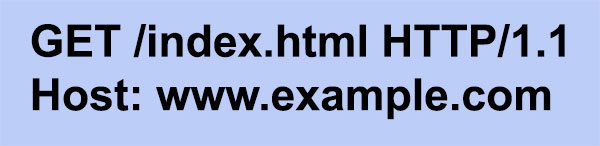
\includegraphics[width=0.3\textwidth]{./04-figuras/fund-teorica/http_exemplo_requisicao}
    \label{fig:exemplorequisicaohttp}
\end{figure}

\begin{figure}[!htb]
    \centering
    \caption{Exemplo de resposta HTTP}
    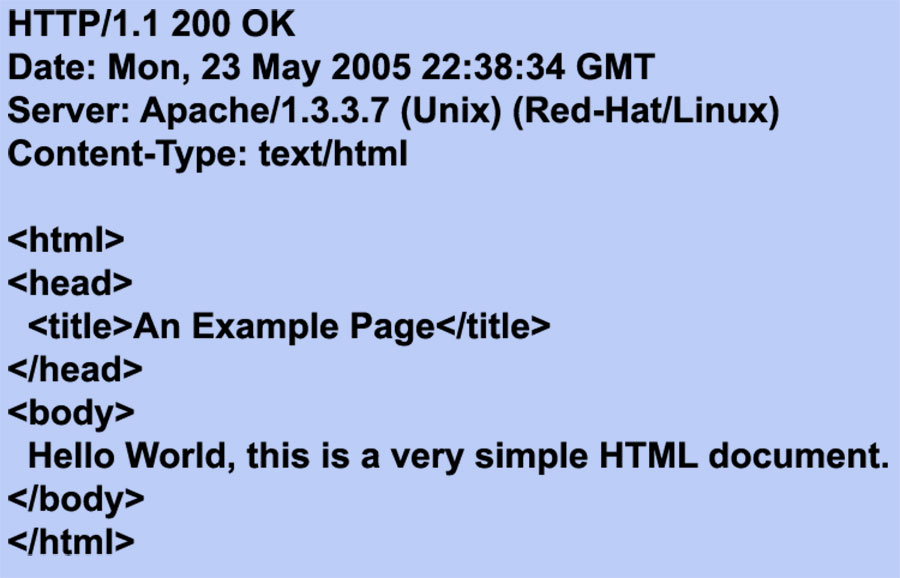
\includegraphics[width=0.5\textwidth]{./04-figuras/fund-teorica/http_exemplo_resposta}
    \label{fig:exemplorespostahttp}
\end{figure}

Apesar de ter sido utilizado desde 1990, o HTTP recebeu sua primeira documentação oficial em 1991, quando recebeu um número de versão e passou a ser chamado de HTTP/0.9. O funcionamento básico do protocolo é explicado por \citeonline{HighPerformanceBrowserNetworking} da seguinte maneira:

\begin{itemize}
	\item Uma conexão TCP era aberta entre o navegador (chamado também de cliente) e o servidor
	\item A requisição do cliente era uma cadeia simples de caracteres ASCII
	\item A resposta do servidor era uma torrente de caracteres ASCII que representava um arquivo HTML
	\item A conexão era fechada após a transferência do documento 
\end{itemize}

Com o passar dos anos, a \textit{World Wide Web} de Tim Berners-Lee cresceu rapidamente e isso fez com que o uso do HTTP aumentasse muito em pouco tempo. Viu-se a necessidade de um protocolo mais robusto e estruturado, mas que mantivesse a simplicidade do HTTP/0.9, pois esta era vista como o motivo por trás do sucesso do protocolo. Então o IETF\footnote{Força Tarefa de Engenharia da Internet, conhecida como IETF na sigla em inglês, é uma comunidade aberta formada por profissionais que se preocupam com a evolução da Internet e por isso procuram formalizar as técnicas utilizadas na rede global de computadores.} passou a coordenar a criação de especificações para o HTTP e criou o HTTP-WG\footnote{Grupo de Trabalho do HTTP, conhecido como HTTP-WG na sigla em inglês, é um grupo formado por profissionais escolhidos pelo IETF para lidar com as especificações do protocolo.} que tinha a função definir as especificações das versões seguintes do protocolo. Em 1996, foi definido o HTTP/1.0 \cite{RFC1945}, em 1999 o HTTP/1.1 \cite{RFC2616} e em 2015 foi aprovada a especificação para o HTTP/2 \cite{HTTP2Spec}.

\section{Visão Geral do Funcionamento do HTTP}
\label{sec:http_visão_geral}

Como descrito por \citeonline[p.~683]{Tanenbaum}, o HTTP é um simples protocolo de requisições e respostas. As requisições e respostas são compostas por um cabeçalho e um conteúdo, e são enviadas do cliente para o servidor. O HTTP é um protocolo independente de estado, ou seja, cada tupla requisição-resposta pode ser tratada de maneira independente, sem que as anteriores e futuras interfiram nela. O modelo, ilustrado na \autoref{fig:httpoverview}, é bem simples e direto, fácil de ser replicado.

\begin{figure}[!htb]
    \centering
    \caption{Visão Geral do Protocolo HTTP}
    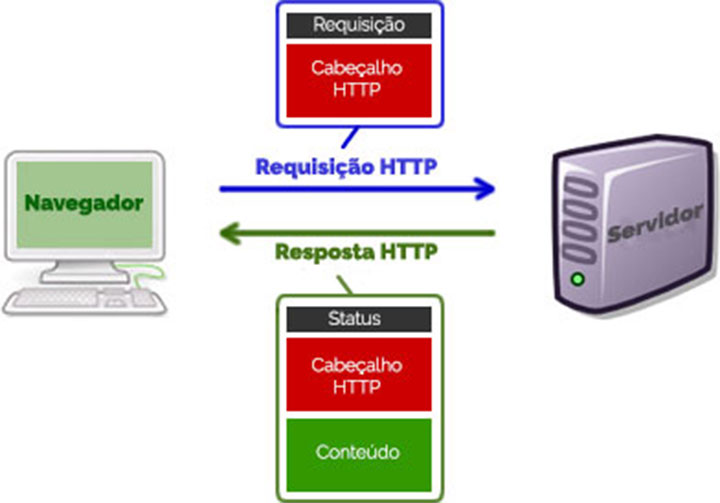
\includegraphics[width=0.6\textwidth]{./04-figuras/fund-teorica/http_overview}
    \fonte{Adaptado de \citeonline{ImagemHTTPOverview}}
    \label{fig:httpoverview}
\end{figure}

O HTTP foi desenvolvido para funcionar como um protocolo de camada de Aplicação em cima do protocolo TCP, conectando as ações do usuário à camada de Apresentação. Contudo, de acordo com \citeonline[p.~684]{Tanenbaum}, ele se transformou em um protocolo da camada de Transporte, criando uma maneira de processos se comunicarem através de diferentes redes. Hoje em dia não são apenas os navegadores \textit{web} que utilizam o protocolo HTTP para se comunicar com servidores: aplicações como tocadores de mídias, anti-vírus, programas de fotos, dentre outras utilizam o HTTP para trocar informações de maneira simples, rápida e eficiente.\cite{Tanenbaum}

Os cabeçalhos HTTP definem características desejadas ou esperadas pelas aplicações e servidores, como tipo de codificação de caracteres ou tipo de compressão dos dados. Existem várias etiquetas padrões que podem ser utilizadas nos cabeçalhos e os desenvolvedores podem ainda criar etiquetas próprias para serem utilizadas dentro das aplicações - por definição, caso um cliente ou servidor receba uma etiqueta que não reconhece ele simplesmente a ignora. No \autoref{qua:cabecalhoshttp} são apresentadas algumas das etiquetas mais utilizadas, mas existem muitas outras que não foram citadas e que podem variar com a versão do protocolo.\cite{Tanenbaum}

\begin{quadro}[!htb]
	\centering
	\caption{Etiquetas para cabeçalhos HTTP.\label{qua:cabecalhoshttp}}
	\begin{tabular}{| c | c | c |}
		\hline
		\textbf{Etiqueta} & \textbf{Tipo} & \textbf{Conteúdo}                                       \\
		\hline
		\textit{Accept}             & Requisição    & Tipo de páginas que o cliente suporta                   \\
		\hline
		\textit{Accept-Encoding}    & Requisição    & Tipo de codificação que o cliente suporta               \\
		\hline
		\textit{If-Modified-Since}  & Requisição    & Data e hora para checar atualidade do conteúdo          \\
		\hline
		\textit{Authorization}      & Requisição    & Uma lista de credenciais do cliente                      \\
		\hline
		\textit{Cookie}             & Requisição    & Cookie definido previamente enviado para o servidor     \\
		\hline
		\textit{Content-Encoding}   & Resposta      & Como o conteúdo foi codificado (e.g. \textit{gzip})               \\
		\hline
		\textit{Content-Length}     & Resposta      & Tamanho da página em \textit{bytes}                              \\
		\hline
		\textit{Content-Type}       & Resposta      & Tipo de \textit{MIME} da página                                  \\
		\hline
		\textit{Last-Modified}      & Resposta      & Data e hora que a página foi modificada pela última vez \\
		\hline
		\textit{Expires}            & Resposta      & Data e hora quando a página deixa de ser válida         \\
		\hline
		\textit{Cache-Control}      & Ambas          & Diretiva de como tratar \textit{cache}                           \\
		\hline
		\textit{ETag}               & Ambas          & Etiqueta para o conteúdo da página                      \\
		\hline
		\textit{Upgrade}            & Ambas          & O novo protocolo para o qual o cliente deseja alterar        \\	
		\hline
	\end{tabular}
	\fonte{Adaptado de \citeonline{Tanenbaum}}
\end{quadro}

O conteúdo de uma resposta HTTP pode assumir diferentes formatos (como, HTML, CSS e JavaScript) e a definição desse formato é feita com a etiqueta \textit{Content-Type} enviada no cabeçalho de resposta. O conteúdo é a maior parte de uma resposta HTTP e os desenvolvedores devem se esforçar para reduzi-lo ao máximo, garantindo que a comunicação de dados seja rápida e eficiente.\cite{Tanenbaum}

Por executar em cima do protocolo TCP, o HTTP precisa que uma conexão TCP seja aberta para poder realizar a troca de dados entre o cliente e o servidor. Como essa conexão é gerenciada depende da versão do protocolo. Após a abertura da conexão, a requisição pode ser enviada. Na primeira linha da requisição, são definidas a versão do protocolo e a operação que será realizada. Apesar de ter sido criado apenas para recuperar páginas \textit{web} de um servidor, o HTTP foi intencionalmente desenvolvido de forma genérica, possibilitando a extensibilidade do seu uso. Sendo assim, o protocolo suporta diferentes operações, chamadas de métodos, além da tradicional requisição de páginas \textit{web} \cite{Tanenbaum}. A lista completa de métodos com suas descrições pode ser vista no \autoref{qua:metodoshttp}. Vale ressaltar que esses métodos são \textit{case sensitive}, ou seja, o método \textit{get}, por exemplo, não existe.

\begin{quadro}[H]
	\centering
	\caption{Métodos HTTP.\label{qua:metodoshttp}}
	\begin{tabular}{| c | c |}
		\hline
		\textbf{Método} & \textbf{Descrição}							 \\
		\hline
		GET             & Ler página \textit{web}					             \\
		\hline
		HEAD            & Ler cabeçalho de página \textit{web}					 \\
		\hline
		POST            & Anexar à página \textit{web}					         \\
		\hline
		PUT             & Armazenar página \textit{web}                            \\
		\hline
		DELETE          & Remover página \textit{web }                             \\
		\hline
		TRACE           & Imprimir requisição de entrada                  \\
		\hline
		CONNECT         & Conectar através de um \textit{proxy}                    \\
		\hline
		OPTIONS         & Listar opções para uma página \textit{web}               \\
		\hline
	\end{tabular}
	\fonte{Adaptado de \citeonline{Tanenbaum}}
\end{quadro}

Dos métodos citados no \autoref{qua:metodoshttp}, GET e POST são os mais utilizados pelos navegadores \textit{web} e serão os mais utilizados neste trabalho. O método GET é utilizado para recuperar informações do servidor e o método POST para enviar informações para o servidor.

Sempre que uma requisição é enviada por um cliente, este recebe uma resposta, mesmo que a requisição não possa ser cumprida pelo servidor, que então enviará uma resposta comunicando o cliente do ocorrido. Na primeira linha do cabeçalho de resposta se encontra o código do estado da resposta em formato numérico de três dígitos. O primeiro digito deste código define a qual sub-grupo ele pertence. O \autoref{qua:estadoshttp} mostra os sub-grupos existentes e o significado de cada um deles. Cada um destes sub-grupos possui vários códigos  com diferentes significados e, com a evolução do protocolo, mais códigos foram sendo inseridos para lidar com necessidades específicas.

\begin{quadro}[!htb]
	\centering
	\caption{Códigos de estado HTTP.\label{qua:estadoshttp}}
	\fonte{Adaptado de \citeonline{Tanenbaum}}
\end{quadro}
\begin{table}[]
\centering
\caption{My caption}
\label{my-label}
\begin{tabular}{|l|l|l|}
\hline
\textbf{Código} & \textbf{Significado} & \textbf{Exemplo}                                                                                   \\ \hline
1xx             & Informação           & \begin{tabular}[c]{@{}l@{}}100 = servidor concorda em lidar\\ com requisição do cliente \end{tabular} \\ \hline
2xx             & Sucesso              & \begin{tabular}[c]{@{}l@{}}200 = sucessona requisição\\ 204 = nenhum conteúdopresente\end{tabular} \\ \hline
3xx             & Redirecionamento     & \begin{tabular}[c]{@{}l@{}}301 = página foi movida\\ 304 = \textit{cache} ainda é válida\end{tabular}       \\ \hline
4xx             & Erro do cliente      & \begin{tabular}[c]{@{}l@{}}403 = página proibida\\ 404 = página não encontrada\end{tabular}        \\ \hline
\end{tabular}
\end{table}
	

A \textit{cache} é uma característica importante do HTTP. O protocolo foi construído com suporte integrado para lidar com este requisito de desempenho. Os clientes e os servidores conseguem gerenciar \textit{caches} com a ajuda dos cabeçalhos de requisição e resposta, mas o tamanho da \textit{cache} é definido pelo navegador. O problema destas memórias locais é saber o momento de utilizar os dados armazenados nelas ou de pedir novos dados ao servidor \cite{Tanenbaum}.

As versões do protocolo HTTP foram corrigindo falhas identificadas quando ele passou a ser utilizado em larga escala. Mas, apesar das mudanças, a essência continua a mesma: um simples protocolo de requisição e resposta.

Nas próximas seções serão, apresentadas comparações entre as versões do HTTP, com ênfase nas mudanças que ajudaram a melhorar a performance dos \textit{websites} e aplicações \textit{web}.

\section{HTTP/1.0 VS HTTP/1.1}
\label{sec:http_10_vs_http_11}

Com a popularização da Internet na década de 1990, o uso do HTTP cresceu rapidamente. Nesse cenário o IETF teve que se apressar para criar um documento de consulta para desenvolvedores que queriam utilizar o protocolo em suas aplicações. Sendo assim, apesar de todo o debate por trás da especificação do HTTP/1.0 \cite{RFC1945}, aprovada em 1996, o documento apenas explicou os usos comuns do protocolo, mas não chegou a definir padrões de como ele deveria ser aplicado, como explica \citeonline{KeyDifferencesHTTP}. Por isso, logo após a sua aprovação, o HTTP-WG já começou a trabalhar na RFC 2616 \cite{RFC2616}, para poder corrigir os erros existentes no HTTP/1.0 com a criação de uma nova versão, o HTTP/1.1.

Várias funcionalidades importantes foram adicionadas no HTTP/1.1, e o HTTP-WG teve o cuidado de manter a compatibilidade entre as versões do protocolo, levando em consideração que o HTTP/1.0 já era amplamente utilizado e não podia se esperar que todos os \textit{websites} e aplicações se adaptassem de uma hora para outra. Esse fato também levou o HTTP-WG a criar um protocolo que fosse flexível a mudanças futuras (lembrando que no HTTP todas as etiquetas que um cliente ou servidor não reconhecem são simplesmente ignoradas). Considerando-se a intensão de se criar um protocolo que possa se estender de acordo com as necessidades do ambiente, as primeiras mudanças no HTTP/1.1 que valem ser citadas foram a criação de duas novas etiquetas para cabeçalhos, \textit{Upgrade} - uma maneira do cliente informar qual versão do protocolo ele suporta - e \textit{Via} - que define uma lista dos protocolos suportados pelos clientes ao longo do caminho de uma transmissã \cite{Tanenbaum}.

Como dito anteriormente, o protocolo HTTP foi construído com suporte integrado para \textit{cache}. Mas o mecanismo de \textit{cache} do HTTP/1.0 era muito simples e não permitia que o cliente ou o servidor definisse instruções diretas de como a memória deveria ser utilizada. O HTTP/1.1 tentou corrigir esse problema com a criação de novas etiquetas para cabeçalhos. A primeira delas é a \textit{ETag}, que define uma cadeia de caracteres única para um arquivo. Além do próprio conteúdo, essa cadeia utiliza a data e a hora da última modificação no arquivo, logo pode ser utilizada para verificar se dois arquivos são idênticos. O HTTP/1.1 também definiu novas etiquetas condicionais para complementar a já existente \textit{If-Modified-Since}. As etiquetas \textit{If-None-Match}, \textit{If-Match} e \textit{If-Unmodified-Since}, passaram a poder ser usadas para verificar se arquivos em \textit{cache} estão atualizados ou não. Uma das mudanças mais significativas no mecanismo de \textit{cache}, foi a etiqueta \textit{Cache-Control} que possibilita definir novas diretrizes para o uso da \textit{cache}, como tempo de expiração relativos e arquivos que não devem ser armazenados \cite{Tanenbaum}.

O HTTP/1.0 tinha muitos problemas em gerenciar a largura de banda. Não era possível enviar partes de arquivos, sendo assim, mesmo se o cliente não precisasse de um arquivo inteiro, ele teria de recebe-lo. No HTTP/1.1, foram então criados a etiqueta \textit{Range}, o tipo \textit{MIME} \textit{multipat/byteranges} e o tipo de compressão \textit{Chuncked} para que cliente e servidores pudessem trocar mensagens com partes de arquivos. Para complementar esse novo mecanismo foi incluído um novo código de resposta, 100, que informava um cliente que o corpo de sua requisição deve ser enviado. Além de poder enviar partes de arquivos, o HTTP/1.1 garante a compressão dos dados durante todo o caminho da transmissão. Nesse sentido, foi incluída a etiqueta \textit{Transfer-Encoding}, que complementa a \textit{Content-Encoding} indicando qual codificação foi utilizada na transmissão ponto a ponto \cite{Tanenbaum}.

O modelo original do protocolo HTTP utilizava uma conexão TCP para cada transmissão. Esse processo era extremamente danoso para o desempenho de \textit{websites} e aplicações, pois se gastava muito tempo na criação e configuração de novas conexões e nos momentos iniciais da conexão (quando, por definição, ela é mais lenta). Para corrigir esse problema, o HTTP/1.1 define conexões persistentes como seu padrão. Conexões persistentes permitem que clientes e servidores assumam que uma conexão TCP continuará aberta após a transmissão de dados, e que esta poderá ser utilizada para uma nova transmissão. Além disso, foi definido que o HTTP/1.1 utilizaria \textit{pipeline}, isto quer dizer que clientes não precisam aguardar a resposta de uma requisição para enviarem uma nova requisição, como era o padrão do HTTP/1.0. Os ganhos com essas novas técnicas podem ser notados na \autoref{fig:httpconexaopersistente} \cite{Tanenbaum}.

\begin{figure}[!htb]
    \centering
    \caption{HTTP com (a) múltiplas conexões e requisições sequenciais. (b) Uma conexão persistente e requisições sequenciais. (c) Uma conexão persistente e requisições em \textit{pipeline}}
    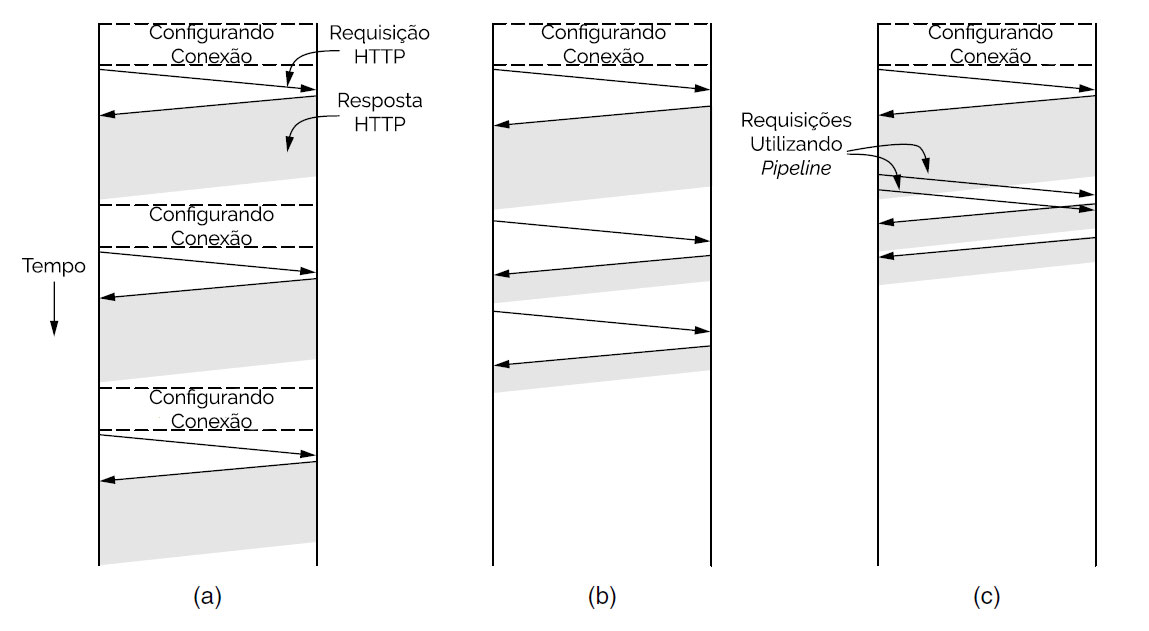
\includegraphics[width=1.0\textwidth]{./04-figuras/fund-teorica/httpconexaopersistente}
    \fonte{Adaptado de  \citeonline{Tanenbaum}}
    \label{fig:httpconexaopersistente}
\end{figure}

Uma funcionalidade desejada no HTTP/1.1 era a de poder fazer requisições para outros servidores além daquele da página principal sendo acessada. Dessa forma desenvolvedores podem hospedar arquivos CSS e JavaScript em um servidor e imagens em outro por exemplo. Isto se tornou possível com a adição da etiqueta \textit{Host}, com a qual o cliente pode definir qual é o caminho do servidor que será utilizado na requisição. Caso a etiqueta \textit{Host} não esteja definida no cabeçalho, é assumido que o caminho do servidor é o caminho da página principal \cite{Tanenbaum}.

Como conclui \citeonline{KeyDifferencesHTTP}: os protocolos HTTP/1.0 e HTTP/1.1 diferem em diversas maneiras. Enquanto muitas dessas mudanças têm o objetivo de melhorar o HTTP, a descrição do protocolo mais do que triplicou de tamanho, e muitas dessas funcionalidades foram introduzidas sem testes em ambientes reais. Esse aumento de complexidade causou muito trabalho para os desenvolvedores de clientes e servidores \textit{web}. 

No \autoref{qua:http11novo} encontra-se um resumo das mudanças introduzidos no protocolo HTTP/1.1.

\begin{quadro}[!htb]
	\centering
	\caption{Mudanças introduzidas no HTTP/1.1.
	\label{qua:http11novo}}
\end{quadro}
\begin{tabularx}{\textwidth}{| X | X |}
	\hline
	\multicolumn{2}{| c |}{\cellcolor[HTML]{C0C0C0}\textbf{Cabeçalhos}} \\
	\hline
	\textbf{Etiqueta} & \textbf{Descrição} \\
	\hline
	\textit{Accept-Encoding}\footnote{A etiqueta \textit{Accept-Encoding} já existia no HTTP/1.0, mas era pouco utilizada por causa da sua especificação confusa, por isso foi redefinida na versão 1.1.} & Lista de codificações aceitas. \\
	\hline
	\textit{Age} & O tempo que o conteúdo está salvo no \textit{proxy} em segundos. \\
	\hline
	\textit{Cache-Control} & Notifica todos os mecanismos de cache do cliente ao servidor se o conteúdo deve ser salvo. \\
	\hline
	\textit{Connection} & Controla a conexão atual. \\
	\hline
	\textit{Content-MD5} & Codificação binária de base-64 para verificar conteúdo da resposta. \\
	\hline
	\textit{ETag} & Identificador único de um conteúdo. \\
	\hline
	\textit{Host} & Indica o endereço e a porta do servidor que deve ser utilizado pela mensagem. \\
	\hline
	\textit{If-Match} & Realize a ação requisitada se, e somente se, o conteúdo do cliente é igual ao conteúdo do servidor. \\
	\hline
	\textit{If-None-Match} & Retorna código 304 se o conteúdo não foi modificado. \\
	\hline
	\textit{If-Range} & Se o conteúdo não foi modificado, envie a parte solicitada, se não, envie o conteúdo novo. \\
	\hline
	\textit{If-Unmodified-Since} & Envie o conteúdo se, e somente se, ele não foi modificado na data esperada. \\
	\hline
	\textit{Keep-Alive} & Detalhes sobre a conexão, tempo que ela ficará aberta e número máximo de requisições aceitas por ela. \\
	\hline
	\textit{Proxy-Authentication} & Pede uma,requisição de autenticação de um \textit{proxy}. \\
	\hline
	\textit{Proxy-Autorization} & Credenciais de autorização para se conectar a um \textit{proxy}. \\
	\hline
	\textit{Range} & Faz a requisição de apenas uma parte de um conteúdo. \\
	\hline
	\textit{Trailer} & Indica que o grupo de cabeçalhos está presente em uma mensagem. \\
	\hline
	\textit{Transfer-Encoding} & A forma de codificação usada para se transferir o conteúdo para o usuário. \\
	\hline
	\textit{Upgrade} & Pede para o servidor atualizar para outro protocolo. \\
	\hline
	\textit{Vary} & Informa quais partes do cabeçalho de requisição devem ser levadas em conta para descobrir se um recurso em \textit{cache} deve ser utilizado ou se este recurso deve ser solicitado no servidor. \\
	\hline
	\textit{Via} & Informa o servidor de \textit{proxies} pelos quais a requisição passou. \\
	\hline
	\textit{Warning} & Mensagem genérica de cuidado para possíveis problemas no corpo da mensagem. \\
	\hline
	\textit{WWW-Authenticate} & Indica tipo de autenticação que deve ser utilizada para acessar entidade requerida. \\
	\hline
	\multicolumn{2}{| c |}{\cellcolor[HTML]{C0C0C0}\textbf{Métodos}} \\
	\hline
	\textbf{Método} & \textbf{Descrição} \\
	\hline
	\textit{OPTIONS} & Solicita informações sobre os recursos que o servidor suporta. \\
	\hline
	\multicolumn{2}{| c |}{\cellcolor[HTML]{C0C0C0}\textbf{Estados}\footnote{Além dos citados ainda foram adicionados outros estados no HTTP/1.1, mas a lista ficaria muito extensa. Logo foram descritos os estados que podem influenciar no desempenho do \textit{front-end}.}} \\
	\hline
	\textbf{Código} & \textbf{Descrição} \\
	\hline
	100 & Confirma que o servidor recebeu o cabeçalho de requisição e que o cliente deve continuar a enviar a mensagem desejada. \\
	\hline
	206 & O servidor está entregando apenas uma parte de um conteúdo por causa da etiqueta de Range na requisição do cliente. \\
	\hline
	300 & Indica as multiplas opções disponíveis para o cliente. \\
	\hline
	409 & Indica que a requisição não pôde prosseguir por causa de um conflito. \\
	\hline
	410 & Indica que o conteúdo requisitado não está mais disponível e não estará disponível no futuro.\\
	\hline
	\multicolumn{2}{| c |}{\cellcolor[HTML]{C0C0C0}\textbf{Diretivas}} \\
	\hline
	\textbf{Diretiva} & \textbf{Descrição} \\
	\hline
	\textit{chuncked} & Utilizado para envio de conteúdo em partes. \\
	\hline
	\textit{max-age} & Determina qual é o tempo máximo que um conteúdo deve ficar salvo em \textit{cache}. \\
	\hline
	\textit{no-store} & Indica que o conteúdo não deve ser salvo em \textit{cache}. \\
	\hline
	\textit{no-transform} & Indica,que o conteúdo não deve ser modificado por \textit{proxies}. \\
	\hline
	\textit{private} & Indica que o conteúdo não deve ser acessado sem autenticação. \\
	\hline
	\multicolumn{2}{| c |}{\cellcolor[HTML]{C0C0C0}\textbf{Tipos de MIME}} \\
	\hline
	\textbf{Tipo} & \textbf{Descrição} \\
	\hline
	\textit{multipart/byteranges} & Indica que o conteúdo que está sendo enviado é apenas uma parte de um todo. \\
	\hline
	\multicolumn{2}{| c |}{\cellcolor[HTML]{C0C0C0}\textbf{Funcionalidades}} \\
	\hline
	\textbf{Nome} & \textbf{Descrição} \\
	\hline
	\textit{Content negotitation} & Escolhe a melhor representação disponível para um conteúdo. \\
	\hline
	\textit{Persistent connection} & Após o termino de uma requisição HTTP a conexão continua aberta e pode ser utilizada por outras requisições. \\
	\hline
	\textit{Pipeline} & O cliente não precisa esperar que a resposta de uma requisição retorne antes de enviar outra requisição. \\
	\hline
\end{tabularx}

\section{HTTP/1.1 VS HTTP/2}
\label{sec:http_11_vs_http_2}

O HTTP/1.1 é robusto e flexível, e isso permitiu que passasse a ser utilizado em aplicações diversas de maneira eficiente. Ao longo dos anos o IETF acrescentou algumas extensões ao protocolo para corrigir erros pontuais, mas o HTTP atendia as necessidades da rede mundial de computadores \cite{Tanenbaum}.

No inicio do século XXI, os \textit{websites} começaram a mudar. Eles se tornaram mais complexos e consequentemente maiores, muitas fontes e folhas de estilo eram utilizadas e cada página passou a possuir vários arquivos de JavaScript. Além disso, eles deixaram de ser estáticos e passaram a responder dinamicamente às ações dos usuários. Hoje em dia, muitas requisições HTTP são necessárias para se montar uma página \textit{web} e essas requisições podem ser longas e demoradas \cite{HighPerformance}.

Esse aumento da complexidade das páginas \textit{web} fez com que o HTTP/1.1 se tornasse um gargalo de desempenho para os \textit{websites}, então em 2007 o IETF formou o grupo HTTPbis (onde o ''\textit{bis}'' quer dizer ''de novo'' em latim). Mas o grupo só começou as discussões sobre a nova versão do protocolo em 2012, terminando de redigir as especificações em 2014. Após revisões, a especificação oficial da nova versão do HTTP foi aprovada no início do ano de 2015 e deve começar a ser utilizada em 2016. A nova versão do HTTP passou a se chamar HTTP/2. As casas decimais, que eram comuns na nomenclatura das outras versões, deixaram de existir agora, caso mudanças sejam necessárias, serão lançadas novas versões do protocolo ao invés de sub-versões.\cite{webPageGrowth}

O HTTP/2 têm o objetivo de corrigir o problema de latência existente na versão anterior. Apesar do sistema de \textit{pipeline}, o HTTP/1.1 é muito sensível à latência, ou seja, apesar de conseguir uma grande quantidade de dados, existem problemas quanto ao tempo de viagem das requisições e respostas. Isso acontece porque o \textit{pipeline} do HTTP/1.1 é muito difícil de ser gerenciado e muitas vezes fecha conexões que deveriam ter ficado abertas. O problema é tão grande que \citeonline{HTTP2Explained} afirma que, mesmo nos dias de hoje, muitos navegadores \textit{web} preferem desativar o \textit{pipeline}. Para corrigir este problema, o HTTP/2 propõe mudanças na forma como as informações são trocadas entre clientes e servidores.

Assim como ocorreu na mudança da versão 1.0 para a versão 1.1, o novo protocolo não deve alterar nenhum paradigma já existente. As aplicações que utilizam o HTTP/1.1 devem continuar funcionando no HTTP/2, os formatos de arquivos, as URL e as URI devem ser mantidos e o usuário final não deve ter de fazer nada para poder aproveitar das melhorias do novo protocolo. Com isso, para tentar criar um protocolo que funcionasse no mundo real tanto quanto no teórico, o HTTPbis decidiu se inspirar no protocolo SPDY. O SPDY \cite{SPDY} é um protocolo para troca de dados entre clientes e servidores \textit{web}. Ele foi criado pela Google em 2010 como uma alternativa ao HTTP.

O SPDY tem como objetivo aumentar a velocidade dos \textit{websites} e aplicações que o utilizam, melhorando o desempenho da \textit{web} como um todo. A escolha de basear o HTTP/2 neste protocolo, veio do fato dele já vir sendo utilizado por várias aplicações ao longo dos anos e ter se provado um conceito funcional e eficiente.

A primeira mudança no HTTP/2 está na forma como ele escreve suas requisições e respostas. Em suas versões anteriores, o protocolo optou por utilizar o formato ASCII para estruturar suas requisições e respostas, mas era difícil separar as partes dos cabeçalhos e tratar espaços em branco indesejados. Para resolver esse problema o HTTP/2 é um protocolo binário. Assim é mais simples quebrar requisições e respostas em quadros, compará-los e comprimir as informações. Entre as desvantagens dessa representação binária estão o fato de que os cabeçalhos HTTP não serão mais compreensíveis sem a ajuda de ferramentas de visualização de pacotes binários e que a depuração do protocolo dependerá de analisadores de pacotes \cite{HTTP2Explained}.

Outro problema muito discutido entre os especialistas em desenvolvimento para a \textit{web} é a segurança da rede. Para garantir a proteção de seus usuário, alguns \textit{websites} e aplicações optam por utilizar serviços de rede seguro via TLS\footnote{https://tools.ietf.org/html/rfc5246}. O TLS é um protocolo que promove a segurança entre as partes envolvidas em comunicações de dados através de autenticação e criptografias. Quando o HTTP é utilizado em conjunto com o TLS, ele recebe o nome de HTTPS. Mas como explica \citeonline[p.~853]{Tanenbaum}, o HTTPS é simplesmente o protocolo HTTP, as diferenças estão no momento do transporte dos dados, quando o protocolo TLS realiza ações para garantir a segurança. Foi muito discutida a ideia de fazer o uso do TLS obrigatório no HTTP/2, mas isto iria forçar todos os \textit{websites} e aplicações a se adaptarem para poderem se adequar ao protocolo. Então, ficou decidido que o uso do TLS continuaria opcional na nova versão \cite{Tanenbaum}.

Utilizando a representação binária, o HTTP/2 possibilita a multiplexação de fluxos de dados. Como explica \citeonline{HTTP2Explained}, um fluxo é uma associação lógica criada por uma sequencia de quadros. No HTTP/2, uma conexão possui vários fluxos e por isso vários componentes podem ser transferidos ao mesmo tempo. Para esse processo funcionar, o protocolo multiplexa esses fluxos no momento do envio e as separa novamente na chegada. A \autoref{fig:streamsmultiplexadas} ilustra a multiplexação de fluxos.

\begin{figure}[!htb]
    \centering
    \caption{Multiplexação de fluxos no HTTP/2 (a) dois fluxos separados (b) fluxos multiplexados}
    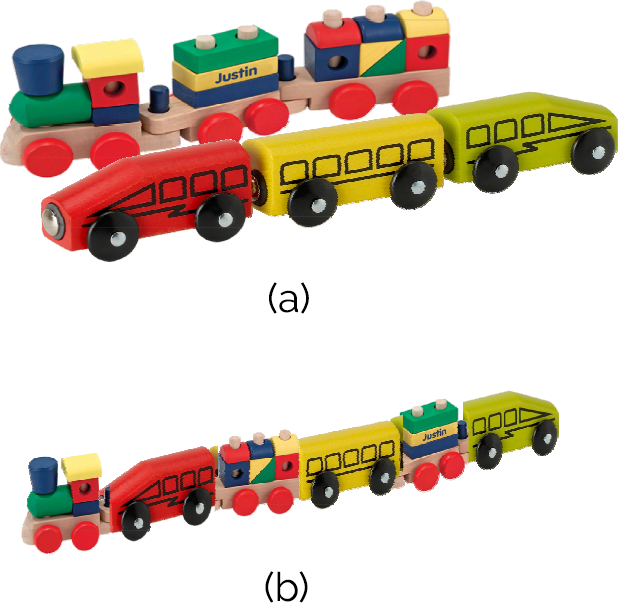
\includegraphics[width=0.5\textwidth]{./04-figuras/fund-teorica/multiplexed_streams}
    \fonte{Adaptado de  \citeonline{HTTP2Explained}}
    \label{fig:streamsmultiplexadas}
\end{figure}

Um problema no HTTP/1.1 era a garantia de que um componente A já teria sido baixado quando outro componente B que depende de A fosse executado. Apesar de o HTML garantir isso, essa limitação impedia que a paralelização de \textit{downloads} fosse maior. No HTTP/2 foram adicionados os mecanismos de prioridade e dependência. Eles tornaram possível indicar quais fluxos devem ser baixados primeiro e quais são suas interdependências. Dessa forma, os desenvolvedores de páginas \textit{web} podem paralelizar ao máximo seus componentes e o protocolo cuidará de evitar erros \cite{HTTP2Explained}.

A compressão de dados é um fator importante para o aumento de desempenho do HTTP. Com o passar dos anos, as requisições e respostas aumentaram de tamanho, e os algoritmos de compressão existentes para o SPDY e o HTTPS não se provaram eficientes contra ataques de terceiros. Logo notou-se que este era um ponto crítico para a nova versão do protocolo, então o HTTPbis decidiu por criar o HPACK, que será o novo formato de compressão para cabeçalhos HTTP/2. Visando a robustez desse formato, foi criada uma nova especificação exclusiva para o HPACK, que detalha como ele funciona e como deve ser usado \cite{HPACKSpec}.

Assim como na versão anterior, o HTTP/2 possui mecanismos para lidar com a \textit{cache}. As etiquetas existentes no HTTP/1.1 continuam a existir, mas uma nova funcionalidade foi adicionada na nova versão, o \textit{Server Push}. O \textit{Server Push} tem o objetivo de permitir que o cliente consiga componentes da maneira rápida, mesmo que seja a primeira vez que ele solicite aquele componente. A \textit{Server Push} funciona da seguinte maneira: o cliente requisita um componente X. O servidor então sabe que é provável que este mesmo cliente vá requisitar o componente Y nos próximos instantes. Sendo assim o servidor pode enviar o componente Y antes mesmo de receber o pedido por ele. Essa funcionalidade é algo que o cliente deverá especificar explicitamente, mas existe grande expectativa quanto às melhorias que ela pode trazer \cite{HTTP2Explained}.

Além dessa melhoria no sistema de \textit{cache}, o HTTP/2 inclui uma nova etiqueta para impedir o desperdício de banda de transmissão. Se o servidor começar a enviar um componente com um tamanho específico e perceber que aquele componente não é mais útil, ele pode cancelar o envio com a etiqueta \textit{RST STREAM}, evitando que o fluxo de envio fique ocupado com dados desnecessários por muito tempo \cite{HTTP2Explained}.

Caso um \textit{website} ou uma aplicação deseje transferir o cliente para outro servidor sem ser o requisitado, ou até mesmo para outra porta, ele poderá utilizar a etiqueta \textit{Alt-Svc}. Com essa etiqueta, o servidor informa ao cliente para onde ele deve ir, então o cliente deve tentar se conectar de maneira assíncrona no caminho sugerido pela \textit{Alt-Svc} e utilizar aquela conexão apenas se ela se provar confiável. Essa etiqueta foi criada com a intensão de informar clientes que os dados requisitados estão disponíveis também em um servidor seguro \cite{HTTP2Explained}.

A escolha pela utilização de envio através de fluxos, tem o objetivo de aumentar a velocidade do protocolo e a quantidade de dados que pode ser enviada de uma só vez. Cada um desses fluxos possui sua própria janela de envio independente, o que garantirá que se um fluxo falhe os outros continuem funcionando. Para impedir o envio de dados e parar todos os fluxos abertos, o protocolo inclui a etiqueta \textit{BLOCKED}, que informa que existem dados para serem enviados, mas algo está impedindo o processo de continuar \cite{HTTP2Explained}.

O protocolo HTTP/2 traz grandes mudanças na estrutura dos dados que serão enviados e recebidos. A essência continua a mesma, um protocolo de requisições e respostas, mas, a medida que o protocolo evolui, novas formas de aprimoramento do desempenhos dos \textit{websites} e das aplicações estão sendo acrescentadas ao HTTP \cite{HTTP2Explained}.

O documento completo com toda a especificação do HTTP/2 pode ser encontrado em \citeonline{HTTP2Spec}. O \autoref{qua:http2novo} mostra um resumo das mudanças detalhadas anteriormente.

\begin{quadro}[!htb]
	\centering
	\caption{Mudanças introduzidas no HTTP/2. \label{qua:http2novo}}
	\begin{tabularx}{\textwidth}{| X | X |}
		\hline
		\textbf{Funcionalidade} & \textbf{Descrição} \\
		\hline
		HTTP/2 binário & Ao invés de utilizar caracteres ASCII para representar informações, o HTTP/2 é binário, o que facilita a comparação de informações, o envio de dados e outras funcionalidades. \\
		\hline
		Fluxos multiplexados & Se existem dois componentes para serem enviados, o protocolo pode optar por multiplexa-los em uma única stream e enviar os dois ao mesmo tempo. \\
		\hline
		Prioridades e dependencias & Caso existam, o cliente pode definir quais componentes possuem prioridade para serem baixados primeiro. Além disso pode informar se existem dependencias entre os  componentes para garantir que quando um arquivo seja baixado todos os outros necessários para o seu funcionamento já estejam no cliente. \\
		\hline
		\textit{HPACK} & Novo sistema de compressão de cabeçalhos para o HTTP/2. \\
		\hline
		RST\_STREAM & Uma maneira de cancelar o envio de componentes. \\
		\hline
		\textit{Server Push} & Habilidade do servidor de enviar um arquivo X para o cliente caso ele veja como provável que o cliente vai precisar desse arquivo no futuro próximo. \\
		\hline
		Janelas individuais de fluxo & Cada fluxo de envio possui sua própria janela que pode ser gerenciada individualmente, assim caso um fluxo falhe os outros continuam. \\
		\hline
		\textit{BLOCKED} & Forma do cliente ou servidor informar a outra parte que existe algo impedindo que o envio de dados continue. \\
		\hline
		Alt-Svc & O servidor pode informa ao cliente de caminhos alternativos para acessar os dados requisitados. \\
		\hline
	\end{tabularx}
\end{quadro}

\newpage
\section{AJAX}
\label{sec:ajax}
AJAX é a sigla em inglês para "Assíncrono JavaScript + XML", e foi inventada por \citeonline{AJAX}. Mas isso não quer dizer que Garrett tenha inventado o modelo AJAX utilizado pelos \textit{websites} e aplicações.

Como dito pelo próprio \citeonline{AJAX}, "AJAX não é uma tecnologia". Na realidade AJAX é a definição de como várias tecnologias podem ser utilizadas em conjunto para ler componentes \textit{web} de maneira assíncrona. Estas tecnologias incluem:
	\begin{itemize}
		\item HTML ou XHTML\footnote{http://en.wikipedia.org/wiki/XHTML}
		\item CSS
		\item JavaScript
		\item DOM\footnote{http://www.w3.org/DOM/}
		\item XML e XSLT\footnote{http://www.w3schools.com/xml/, http://www.w3schools.com/xsl/}
		\item Requisições XMLHttp (\textit{XMLHttpRequest})\footnote{https://developer.mozilla.org/en-US/docs/Web/API/XMLHttpRequest}
	\end{itemize}

A \autoref{fig:compajax} mostra uma comparação entre o modelo clássico de chamadas \textit{web} e o modelo utilizando AJAX. O modelo AJAX adiciona uma camada intermediária entre o usuário e o servidor.

Quando o usuário interage com a página \textit{web}, ele manda uma mensagem para essa nova camada, desenvolvida em JavaScript, que é responsável por requisitar do servidor somente os dados necessários para a interação do usuário e atualizar apenas a parte da página necessária para terminar essa interação. Dessa forma, o AJAX impede que as páginas tenham de ser inteiramente recarregadas a cada interação e consegue melhorar a experiência do usuário \cite{AJAX}.

\begin{figure}[!htb]
    \centering
    \caption{Comparação entre modelo de \textit{web} original e modelo utilizando AJAX}
    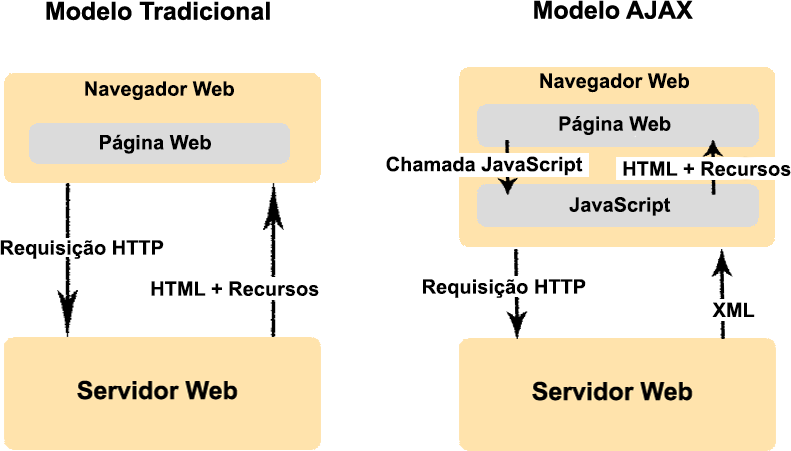
\includegraphics[width=0.7\textwidth]{./04-figuras/fund-teorica/comparacao_ajax}
    \fonte{Adaptado de \citeonline{FigAjax}}
    \label{fig:compajax}
\end{figure}


\section{Web 2.0}
\label{sec:web20}
A \textit{Web} 2.0 não é uma nova versão da \textit{World Wide Web} criada por Tim Berners-Lee. Como explica \citeonline{Web20}, o termo \textit{Web} 2.0 surgiu de uma discussão entre a companhia de mídia O'Reilly e a empresa de produção de MediaLive, quando estavam preparando uma conferencia sobre a \textit{Web}. O que eles chamaram de \textit{Web} 2.0 foi a nova forma como a criação de Berners-Lee estava sendo utilizada pelas pessoas.

O desenvolvimento de técnicas AJAX e o conceito de conhecimento coletivo fez com que a \textit{Web} deixasse de ser utilizada apenas para mostrar páginas estáticas e passasse a explorar a interação com o usuário. Sendo assim \textit{websites} se tornaram aplicações \textit{web}, que melhoravam à medida que os usuários iam alimentando-as com novas informações. Como exemplo de aplicações que exploram os conceitos definidos na \textit{Web} 2.0 podemos citar a Wikipedia \footnote{https://www.wikipedia.org/}, o Facebook \footnote{https://www.facebook.com/} e o Google Maps \footnote{https://www.maps.google.com/}. Todas essas aplicações utilizam de técnicas AJAX para garantir uma boa experiência e são alimentadas com informações entradas pelos usuários, o que as torna mais dinâmicas e flexíveis do que os \textit{websites} da \textit{Web} 1.0 (como ficou conhecida a primeira fase da \textit{Web}) \cite{Web20}.          	% Fundamentação teórica
    %
% Documento: Trabalhos Relacionados
%

\chapter{Trabalhos Relacionados}
Desenvolvedores estão sempre a procura de maneiras para tornar suas aplicações mais rápidas aos olhos dos usuários finais e isso não é diferente com os \textit{websites}. A área de otimização de desempenho para páginas \textit{web} é tão antiga quanto a \textit{World Wide Web}, mas por muito tempo os esforços foram dedicados à otimização de \textit{back-end}, o que \citeonline{HighPerformance} provou não ser o melhor caminho para se atingir o objetivo desejado.

De acordo com \citeonline[p.~5]{HighPerformance}: "Apenas 10-20\% do tempo de resposta do usuário final são gastos baixando o documento HTML. Os outros 80-90\% são gastos baixando todos os componentes da página.". Então, os desenvolvedores podem obter melhores resultados de desempenho caso foquem seus esforços na otimização do \textit{front-end} de seus \textit{websites} ao invés do \textit{back-end}.

Neste capítulo são apresentadas as ideias principais dos dois livros  de Steve Souders. Esses livros tornaram o conhecimento sobre a otimização de desempenho de \textit{front-end} de \textit{websites} acessível a todos os desenvolvedores e ajudaram a melhorar a \textit{web} nos últimos anos.

\section{\textit{High Performance Web Sites}}
\label{sec:highperformancewebsites}

No livro \textit{High Performance Web Sites} \cite{HighPerformance}, Steve Souders descreve 14 regras para a otimização de desempenho de \textit{front-end} de \textit{websites}. De acordo com \citeonline[p.~5]{HighPerformance}: "Se você seguir todas as regras aplicáveis a seu \textit{website}, você vai fazer sua página 25-50\% mais rápida e melhorar a experiência do usuário.". As regras são muito variadas e contemplam de configurações básicas de servidores, a redução do tamanho de arquivos e melhores práticas de programação.

A seguir, serão explicadas as 14 regras encontradas no livro, ordenadas, de acordo com Steve Souders, das que causam maior impacto no desempenho às que causam menor impacto.

\subsection{Regra 1: Faça menos requisições HTTP}
\label{subsec:highperformance_regra1}
Cada componente de uma página \textit{web} gera pelo menos uma requisição e uma resposta HTTP para chegar do servidor ao cliente. Essas chamadas HTTP costumam ser um grande gargalo de desempenho para \textit{websites} e aplicações \textit{web}, pois como explicou Souders, 80-90\% do tempo de montagem dessas páginas é gasto baixando outros componentes além do HTML. Assim, uma solução para diminuir o tempo de resposta para o usuário final é diminuir o número de componentes que precisam ser baixados. Com esse objetivo, as seguintes técnicas devem ser utilizadas:
	\begin{itemize}
		\item CSS\textit{Sprites} \footnote{http://www.w3schools.com/css/css\_image\_sprites.asp}
		\item \textit{Inline images}
		\item Combinar \textit{scripts} e folhas de estilo\footnote{A técnica não sugere a união de \textit{scripts} com folhas de estilo, e sim \textit{scripts} com \textit{scripts} e folhas de estilo com folhas de estilo, diminuindo o número de arquivos existentes.}
	\end{itemize}

\subsection{Regra 2: Use Redes de Entrega de Conteúdo (CDN)}
\label{subsec:highperformance_regra2}
No HTTP/1.1, o número de conexões TCP que os navegadores \textit{web} abrem em paralelo no mesmo domínio é limitado, com o objetivo de garantir a qualidade de cada conexão. Apesar de esse número ser maior que no HTTP/1.0, o limite continua existindo. Outra característica dessas conexões é que elas são afetadas pela distância física entre clientes e servidores, logo, um usuário que esteja no Brasil vai demorar mais para acessar componentes que estejam hospedados na China do que componentes que estejam hospedados nos Estados Unidos. Uma maneira de resolver esses dois problemas simultaneamente são as CDNs \footnote{http://en.wikipedia.org/wiki/Content\_delivery\_network}. Ao invés de hospedar todos os componentes do \textit{website} no mesmo servidor, os desenvolvedores deveriam utilizar das CDNs para garantir maior paralelismo e diminuir as distâncias geográficas entre seus sistemas e seus usuários.

\subsection{Regra 3: Adicione cabeçalhos de expiração}
\label{subsec:highperformance_regra3}
O HTTP foi desenvolvido com suporte nativo para gerenciamento de \textit{cache}. Mas para essa \textit{cache} funcionar de maneira eficiente, é necessário que os desenvolvedores configurem seus servidores para informar aos navegadores \textit{web} que certos arquivos devem ficar salvos localmente. A maneira de garantir que os arquivos serão salvos em \textit{cache}, é o envio da etiqueta \textit{Expires} no cabeçalho HTTP da resposta que possui o arquivo. Essa configuração não é definida por padrão nos servidores, então os desenvolvedores devem analisar quais arquivos devem utilizar desse recurso e por quanto tempo eles serão válidos. A \textit{cache} é uma ferramenta muito importante na otimização de desempenho, e deixar de usa-la causa grandes danos no tempo médio de resposta de \textit{websites} e aplicações \textit{web}.

\subsection{Regra 4: Utilize \textit{gzip} nos componentes}
\label{subsec:highperformance_regra4}
De acordo com \citeonline[p.~29]{HighPerformance}, essa é a técnica mais simples e que causa maior efeito no tamanho em \textit{bytes} das páginas \textit{web}. O HTTP e os navegadores \textit{web} possuem suporte para compressão de todos os tipos de arquivos, os desenvolvedores só precisam garantir que os clientes e os servidores informem uns aos outros que a esse mecanismo está habilitado. Para fazer isso, a etiqueta de cabeçalho \textit{Accept-Encoding} deve ser definida com os formatos de compressão suportados. O \textit{gzip} é um formato de compressão criado especialmente para a \textit{web} e é o mais eficiente para ser utilizado no HTTP.

\subsection{Regra 5: Coloque folhas de estilo no topo da página}
\label{subsec:highperformance_regra5}
Como disse \citeonline[p.~38]{HighPerformance}, "essa regra tem menos a ver com melhorar o tempo de carregamento da página e mais a ver com como o navegador \textit{web} reage à ordem dos componentes.". Por definição, os navegadores não mostram os elementos da tela até que todas as folhas de estilo tenham sido carregadas, para evitar erros de desenho. Sendo assim, os desenvolvedores devem colocar as folhas de estilo no topo da página (de preferência, dentro do elemento HTML \textit{<head></head>}\footnote{http://www.w3schools.com/tags/tag\_head.asp}), pois elas devem ser os primeiros componentes a serem baixados.

\subsection{Regra 6: Coloque \textit{scripts} no fim da página}
\label{subsec:highperformance_regra6}
Ao contrário das folhas de estilo, os arquivos de \textit{script} devem ser colocados no final do arquivo HTML. Componentes localizados abaixo de arquivos de \textit{script} são bloqueados de serem baixados e desenhados até que o \textit{script} tenha terminado de ser carregado. Isso porque o navegador quer garantir que o \textit{script} esteja pronto caso ele vá executar alguma alteração no restante da página.

\subsection{Regra 7: Evite expressões CSS}
\label{subsec:highperformance_regra7}
Apesar de já não serem suportadas na maioria dos navegadores \textit{web}, os desenvolvedores não devem utilizar expressões CSS em nenhum caso, mesmo nos casos em que o navegador oferece essa alternativa. Esse tipo de expressão é calculada toda vez que há uma movimentação na página (desenhos de novos componentes, uso da barra de rolagem, dentre outros) e isso pode afetar, em muito, o desempenho de um \textit{website} ou aplicação \textit{web}.

\subsection{Regra 8: Faça arquivos \textit{JavaScript} e folhas de estilo externos}
\label{subsec:highperformance_regra8}
Existem duas maneiras de incluir estilos e \textit{scripts} em um \textit{website} ou em uma aplicação \textit{web}. A primeira delas é inserir blocos de código em linha, ou seja, colocar os código diretamente no arquivo HTML, de preferência seguindo as Regras 5 e 6. Apesar de funcionar, essa maneira impede um bom uso da \textit{cache}, porque arquivos HTML geralmente não são salvos em \textit{cache}, logo, os estilos e \textit{scripts} têm de ser baixados todas as vezes que a página é carregada. Levando em consideração que a Regra 3 está sendo usada, uma maneira mais eficiente se inserir estilos e \textit{scripts} em uma página é colocando-os em arquivos externos e adicionando os arquivos no HTML. Dessa forma, os arquivos externos podem ser salvos em \textit{cache} e não precisam ser baixados todas as vezes que o HTML é requisitado.

\subsection{Regra 9: Reduza o número de pesquisas de DNS}
\label{subsec:highperformance_regra9}
Usar diferentes domínios para hospedar componentes é uma maneira de possibilitar que esses componentes sejam baixados em paralelo. Mas a pesquisa por domínios é cara e pode acabar influenciando no tempo de carregamento de uma página. Por isso, os navegadores salvam os domínios cujo o IP já conhecem em \textit{cache}. Levando em consideração esse custo de pesquisa, existe um limite para até quando hospedar componentes em domínios diferentes é benéfico. Os desenvolvedores têm que analisar a quantidade de pesquisas de DNS para domínios únicos (que não estão em \textit{cache}) que estão sendo feitas no carregamento da página e decidir se ainda vale a pena aumentar o paralelismo. Como regra geral, os desenvolvedores deveriam distribuir seus componentes em pelo menos dois e no máximo quatro domínios.

\subsection{Regra 10: Minimizar componentes}
\label{subsec:highperformance_regra10}
Minimizar é a técnica de reduzir caracteres desnecessários de códigos. Essa técnica pode ser utilizada para qualquer tipo de arquivo CSS, JS, HTML, dentre outros. A minimização reduz o tempo de carregamento de páginas \textit{web} porque reduz o tamanho do arquivo diminuindo o tempo gasto para baixa-lo.

\subsection{Regra 11: Evite redirecionamentos}
\label{subsec:highperformance_regra11}
Redirecionamentos são situações em que o usuário tenta acessar uma página \textit{web} e essa página o informa que ele deve ser encaminhado para outra página. Os redirecionamentos são feitos através dos códigos da família 3xx do protocolo HTTP, sendo que os diferentes códigos dessa família informam a razão para o redirecionamento.

Redirecionamentos são extremamente danosos para a experiência de uso de \textit{websites} e aplicações \textit{web}, pois nada é mostrado para o usuário até que o redirecionamento seja concluído e o conteúdo HTML termine de ser carregado. Logo, desenvolvedores não devem utilizar redirecionamento, a não ser em casos em que sejam indispensáveis.

\subsection{Regra 12: Remova \textit{scripts} duplicados}
\label{subsec:highperformance_regra12}
Em projetos grandes, é comum que vários desenvolvedores façam alterações no código e isso pode fazer com que um mesmo arquivo seja inserido mais de uma vez em uma página HTML. \textit{Scripts} duplicados aumentam o número de chamadas HTTP e isso é muito prejudicial ao desempenho de \textit{websites} e aplicações \textit{web}. Sendo assim os desenvolvedores devem ser muito cuidadosos quanto aos \textit{scripts} que estão sendo carregados em suas páginas e ter certeza de que todos são únicos e necessários.

\subsection{Regra 13: Configure \textit{ETags}}
\label{subsec:highperformance_regra13}
Muitas vezes os desenvolvedores não configuram como funcionará o mecanismo de \textit{ETags} de seus servidores e isso pode fazer com que o mecanismo de \textit{cache} seja prejudicado. Como o valor do \textit{ETag} de um componente é único para cada servidor, se o cliente requisitar um componente no servidor X e mais tarde requisitar o mesmo componente no servidor Y, mesmo que este tenha sido salvo na \textit{cache} do navegador na primeira vez, ele será baixado novamente. Na maioria das vezes é melhor desabilitar a opção de \textit{ETags} do que correr o risco de influenciar negativamente no sistema de \textit{cache}.

\subsection{Regra 14: Habilite \textit{cache} para AJAX}
\label{subsec:highperformance_regra14}
As chamadas AJAX melhoram muito a experiência do usuário, pois tornam as páginas \textit{web} mais dinâmicas e responsivas. O problema é que muitas vezes elas não são salvas em \textit{cache} e isso pode afetar o desempenho dos \textit{websites} e aplicações \textit{web}. Para garantir que as chamadas AJAX serão salvas em \textit{cache}, os desenvolvedores devem seguir seguir as regras 1 a 13 também para esse tipo de componente, tomando cuidado especial com a regra 3.


\section{\textit{Even Faster Web Sites}}
\label{sec:evenfasterwebsites}

Com o objetivo de difundir ainda mais as técnicas de otimização para \textit{front-end} de \textit{websites}, Steve Souders lançou, em 2009, seu segundo livro, intitulado \textit{Even Faster Web Sites} \cite{HighPerformance}. Nesta obra, o autor teve a contribuição de outros 8 profissionais da área de otimização que escreveram 6 dos 14 capítulos do livro.

As técnicas descritas em \textit{Even Faster Web Sites} são mais avançadas, e, consequentemente, mais difíceis de serem aplicadas do que as da obra anterior. Além disso, elas não vêm em formato de regras a serem seguidas, o que facilitava a aplicação das regras descritas em \textit{High Performance Web Sites}. Alguns capítulos do livro explicam melhores técnicas de programação, descrevem o funcionamento de mecanismos da \textit{web} e outros ainda reforçam ideias anteriores.

Nesta seção, são resumidas as ideias principais de cada capítulo.

\subsection{Entendendo desempenho em AJAX}
\label{subsec:evenfaster_cap1}
Para saber se vale a pena otimizar o desempenho de um \textit{website} ou de uma aplicação \textit{web}, os desenvolvedores devem levar em conta o tempo e o esforço que deverão ser empregados no processo de otimização, e conhecer quanto essa otimização pode melhorar a experiência do usuário. Desta forma, pode-se decidir se compensa fazer um investimento nesse processo. O desenvolvedor deve se lembrar que otimizar componentes que não têm contribuição expressiva no tempo de carregamento de uma página \textit{web} não é muito relevante para a experiencia do usuário.

Os componentes AJAX representam parte importante das aplicações na \textit{Web} 2.0. Esses componentes são carregados enquanto o usuário está navegando na página, então deve-se evitar qualquer cenário em que a aplicação congele à espera da resposta de uma requisição AJAX. Os desenvolvedores devem identificar quais componentes compensam ser otimizados utilizando os "Eixos do Erro", descrito por \citeonline[p.~2]{EvenFaster} e focar seus esforços nesse componentes.

Durante o processo de otimização de componentes AJAX, os desenvolvedores devem se lembrar:
\begin{itemize}
	\item A maior parte do tempo do navegador é gasta na construção do DOM e não no \textit{JavaScript}.
	\item Códigos organizados são mais fáceis de serem otimizados.
	\item Iterações afetam muito o desempenho de uma aplicação \textit{web}.
	\item Truques (\textit{tricks}) não compensam, a não ser que eles se provem realmente eficientes.
\end{itemize}

\subsection{Criando aplicações \textit{web} responsivas}
\label{subsec:evenfaster_cap2}
Aplicações responsivas são aquelas que respondem ao usuário de maneira rápida e eficiente, fazendo com que ele não sinta que está esperando\footnote{O termo ''página responsiva'' pode ser utilizado em dois contextos. O primeiro é a responsividade com relação ao desempenho da página, ou seja, o tempo que ela demora para responder. O segundo se refere a responsividade do \textit{layout} da página, ou seja, a habilidade que ela tem de se adaptar à diferentes tamanhos de tela.}. Atrasos maiores do que 0,2 segundos causam no usuário a sensação de que o navegador está tendo problemas para conseguir sua resposta, e isso afeta sua experiência de uso. O mecanismo responsável pela responsividade das aplicações é o AJAX.

Em aplicações grandes, muitas chamadas AJAX pode ser executadas ao mesmo tempo e isso é um problema para o \textit{JavaScript}. De acordo com Brendan Eich, criador do \textit{JavaScript}, sua linguagem não possui e nunca vai possuir \textit{threads}. Assim, fica por responsabilidade dos desenvolvedores, encontrar técnicas para melhorar o paralelismo de suas aplicações.

\subsection{Dividindo carga inicial}
\label{subsec:evenfaster_cap3}
O tempo inicial de carregamento de uma página é um fator muito importante na otimização de desempenho. Usuários não gostam de esperar para poder interagir com uma aplicação ou \textit{website} e a grande maioria desses usuários desiste de esperar se o tempo for muito longo. Sendo assim, os desenvolvedores devem definir quais métodos de seus \textit{scripts} são necessários no evento \textit{onload} (evento executado assim que a página é carregada) e separa-los em arquivos diferentes dos outros métodos. Os métodos que devem ser executados logo que a página for carregada devem ser declarados no início do documento HTML. Os outros podem ser declarados ao final da página ou até mesmo de maneira assíncrona.

\subsection{Carregando \textit{scripts} sem bloqueios}
\label{subsec:evenfaster_cap4}
\textit{Scripts} possuem um efeito muito negativo no carregamento de páginas. Enquanto estão sendo baixados e executados, eles bloqueiam o carregamento de componentes localizados abaixo deles. Então, é muito importante definir quais \textit{scripts} podem ser baixados independentes do resto da página e encontrar maneiras de requisitar esses \textit{scripts} sem bloquear o resto da página. No Capítulo 4 deste livro, \citeonline{EvenFaster} descreve seis técnicas de como carregar arquivos de \textit{script} externos de forma assíncrona:

\begin{itemize}
	\item \textit{XHR Eval}, \cite[p.~29]{EvenFaster}
	\item \textit{XHR Injection}, \cite[p.~31]{EvenFaster}
	\item \textit{Script in Iframe}, \cite[p.~31]{EvenFaster}
	\item \textit{Script in DOM Element}, \cite[p.~32]{EvenFaster}
	\item \textit{Script Defer}, \cite[p.~32]{EvenFaster}
	\item \textit{document.write Script Tag}, \cite[p.~33]{EvenFaster}
\end{itemize}

Não existe uma solução única para todos os \textit{websites} e aplicações \textit{web}, então os desenvolvedores devem analisar qual é a melhor para sua situação específica. E caso seja definido que a página terá de ser congelada por algum tempo, os desenvolvedores devem se certificar de que algum indicador de navegador ocupado está sendo mostrado ao usuário\footnote{http://www.stevesouders.com/blog/2013/06/16/browser-busy-indicators/}.

\subsection{Lidando com \textit{scripts} assíncronos}
\label{subsec:evenfaster_cap5}
Quando as técnicas descritas no Capítulo 4 \cite[p.~27]{EvenFaster} são utilizadas para carregar \textit{scripts} sem bloqueios, cria-se um novo problema. Componentes que são carregados de maneira assíncrona estão sujeitos a condições de corrida\footnote{http://en.wikipedia.org/wiki/Race\_condition}. Essas condições tornam imprevisível a ordem na qual os \textit{scripts} serão carregados, o que pode fazer com que ocorram falhas nas dependências de funções. Para evitar essas falhas, Steve Souders descreve 5 técnicas de como garantir que os \textit{scripts} serão carregados em uma ordem na qual sejam executados sem erros de dependências:

\begin{itemize}
	\item \textit{Hardcoded Callback}, \cite[p.~46]{EvenFaster}
	\item \textit{Windows Onload}, \cite[p.~47]{EvenFaster}
	\item \textit{Timer}, \cite[p.~48]{EvenFaster}
	\item \textit{Script Onload}, \cite[p.~49]{EvenFaster}
	\item \textit{Degrading Script Tags}, \cite[p.~50]{EvenFaster}
\end{itemize}

Ao final do capítulo, Souders ainda descreve uma técnica que chamou de "Solução Geral" \cite[p.~59]{EvenFaster}.

\subsection{Posicionando blocos de \textit{scripts} em linha}
\label{subsec:evenfaster_cap6}
Apesar de não gerarem novas requisições HTTP, blocos de \textit{scripts} em linha, ou seja, aqueles posicionados dentro do documento HTML, bloqueiam outros componentes de serem carregados enquanto eles estão sendo executados e isso impede o desenho progressivo da página. Para evitar esse efeito, blocos de \textit{scripts} em linha devem ser movidos para o final da página e, se possível, serem executados de maneira assíncrona. Outro grave problema com esse tipo de \textit{script} é que, quando eles são antecedidos por folhas de estilo, eles não começam a executar enquanto os estilos não são carregados. Dessa forma, é uma boa técnica não colocar blocos de \textit{scripts} em linha logo após chamadas de folhas de estilo.

\subsection{Escrevendo códigos \textit{JavaScript} eficientes}
\label{subsec:evenfaster_cap7}
Neste capítulo, Nicholas Zakas descreve boas técnicas de programação para códigos \textit{JavaScript} que visam otimizar o desempenho do código. As técnicas descritas são:

\begin{itemize}
	\item Melhorar gerenciamento de escopos, \cite[p.79]{EvenFaster}
	\item Use variáveis locais, \cite[p.~81]{EvenFaster}
	\item Otimize acesso a dados frequentes, \cite[p.~85]{EvenFaster}
	\item Use condicionais mais eficientes, \cite[p.~89]{EvenFaster}
	\item Use iterações mais eficientes, \cite[p.~93]{EvenFaster}
	\item Otimize cadeias de caracteres, \cite[p.~99]{EvenFaster}
	\item Evite função com tempo de execução longo, \cite[p.~102]{EvenFaster}
	\item Habilite contadores de tempo, \cite[p.~103]{EvenFaster}
\end{itemize}

\subsection{Escalando usando \textit{Comet}}
\label{subsec:evenfaster_cap8}
Quando muitos dados precisam ser entregues de maneira assíncrona, o mecanismo de AJAX pode acabar causando um problema conhecido como \textit{long-polling} de requisições. \textit{Long-polling} ocorre quando muitas chamadas ao servidor são feitas em um curto intervalo de tempo e o servidor não consegue responder todas no tempo desejado, então algumas dessas chamadas falham, ou ficam muito tempo paradas. \textit{Comet} é um termo que se refere a uma coleção de técnicas, protocolos e implementações que tem como objetivo melhorar o tráfego de dados em baixa latência\footnote{http://ajaxexperience.techtarget.com/images/Presentations/Carter\_Michael\_ScalableComet.pdf}.

\subsection{Indo além do \textit{gzip}}
\label{subsec:evenfaster_cap9}
Mesmo com o suporte à compressão de dados com \textit{gzip} habilitado nos \textit{websites} e aplicações, uma média de 15\% dos usuários continua recebendo dados sem compressão alguma. A maior causa disso são os \textit{proxies} e os programas de anti-vírus. Esses sistemas modificam os cabeçalhos HTTP para poderem ter acesso aos dados que estão sendo enviados a fim de realizarem suas tarefas de inspeção do conteúdo trafegado.

Se essas entregas sem compressão fossem dissolvidas entre todos os usuários da página \textit{web}, o problema seria menos relevante. Mas o que ocorre é que os mesmos 15\% dos usuário estão sempre acessando os \textit{websites} e aplicações de forma mais lenta, o que acaba com a experiência desses usuários e os desencoraja a voltar a acessar a página.

Considerando este fato, Tony Gentilcore, reforça as ideias expostas por Steve Souders no livro \textit{High Performance Web Sites}, \cite{HighPerformance}, de que os desenvolvedores devem fazer seus arquivos os menores possíveis e reduzir o número de chamadas HTTP.

\subsection{Otimizando imagens}
\label{subsec:evenfaster_cap10}
Imagens são consideradas ótimos componentes para se conseguir melhora de desempenho sem ter de abrir mão de funcionalidades. Existem vários padrões de formato para imagens\footnote{http://en.wikipedia.org/wiki/Image\_file\_formats}, cada um deles é determinado pelo tipo de compressão que usa e cada um deles possui seus prós e contras. Sendo assim, os desenvolvedores devem decidir que tipo de qualidade que eles desejam em suas imagens, então selecionar o formato que se adeque às suas necessidades e otimizar essas imagens o máximo possível.

Como regra geral, os desenvolvedores devem optar por utilizar o formato PNG sempre que possível.

\subsection{Quebrando domínios dominantes}
\label{subsec:evenfaster_cap11}
Mesmo que isso aumente a quantidade de pesquisas de DNS, muitas vezes aumentar o número de domínios nos quais componentes estão hospedados melhora o desempenho de \textit{websites} e aplicações \textit{web}. O motivo disso é que mais componentes podem ser baixados em paralelo, o que diminui o tempo total de carregamento da página. O desafio é encontrar o número de domínios que resulta no menor tempo de carregamento da página. Como regra geral, \citeonline[p.~168]{EvenFaster} determina que dividir componentes entre dois a quatro domínios gera resultados satisfatórios.

\subsection{Entregando o documento cedo}
\label{subsec:evenfaster_cap12}
Por padrão, uma página \textit{web} só começa a baixar os seus componentes depois que o documento HTML é totalmente carregado. Sendo assim, durante algum tempo, a única atividade que está sendo realizada pelo navegador é a espera do carregamento do documento HTML. Contudo, existem técnicas para diminuir esse tempo de espera e, consequentemente, o tempo de carregamento de uma página.

Uma boa prática é entregar o documento HTML em partes para o navegador, desde que essas partes possam acelerar o processo de carregamento. Para isso, Steve Souders sugere que o cabeçalho HTML, onde normalmente são declaradas as folhas de estilo, seja entregue assim que estiver pronto. Dessa forma, o navegador pode começar a baixar esses componentes antes mesmo que o carregamento do HTML esteja concluído. Essa técnica é possível graças à etiqueta \textit{Chuncked Encoding}, adicionada no HTTP/1.1, e às funções de carregamento parcial de arquivos em fluxos de dados presentes em algumas linguagens de \textit{back-end} como PHP e NodeJS.

\subsection{Usando \textit{Iframes} com moderação}
\label{subsec:evenfaster_cap13}
Os \textit{Iframes} são componentes HTML que permitem incorporar documentos dentro de outros documentos. Apesar de terem sido muito utilizados no passado, principalmente para adicionar publicidades a \textit{websites}, os \textit{Iframes} são pouco usados nos dias de hoje. A razão disso é que são componentes muito pesados e que bloqueiam o desenho das páginas \textit{web}.

Como regra geral, Steve Souders aconselha não utilizar estes componentes.

\subsection{Simplificando seletores CSS}
\label{subsec:evenfaster_cap14}
Na \textit{Web} 2.0, folhas de estilo são tão populares quanto \textit{scripts}. \textit{Websites} possuem várias folhas de estilo, mas pouco esforço é empregado em otimizar esses arquivos.

Neste capítulo, Souders explica que os navegadores fazem buscas por componentes declarados em folhas de estilo da direita para esquerda, logo os identificadores mais à direita devem ser os mais específicos, para diminuir o tempo de busca. Além disso ele alerta para o mal de códigos duplicados e cita boas práticas de programação para CSS \cite[p.~195]{EvenFaster}.

\section{Análise das técnicas propostas}
Conhecendo as técnicas de otimização de desempenho propostas por Souders para o HTTP/1.1, este trabalho analisa o comportamento de tais técnicas quando aplicadas em \textit{websites} que utilizam o HTTP/2. Como as duas versões do protocolo apresentam mudanças significativas, espera-se que o comportamento das técnicas explicadas até o momento sofram alterações significativas.
     	% Trabalhos relacionados
    %
% Documento: Metodologia
%

\chapter{Metodologia}
\label{chap:metodologia}

Para alcançar os objetivos propostos de entender o funcionamento das técnicas de otimização propostas por Steve Souders em seus dois livro, \textit{High Performance Web Sites}, \cite{HighPerformance}, e \textit{Even Faster Web Sites}, \cite{EvenFaster}, quando aplicadas ao HTTP/2 e, se necessário, propor novas técnicas para essa versão do protocolo, este trabalho foi divido em quatro etapas:

\begin{itemize}
	\item Etapa 1: Seleção das técnicas de melhora de desempenho;
	\item Etapa 2: Preparação dos testes das técnicas selecionadas;
	\item Etapa 3: Realização dos teste e coleta de dados;
	\item Etapa 4: Análise dos resultados.
\end{itemize}

Neste capítulo serão descritas as etapas deste trabalho.

\section{Seleção das técnicas de melhora de desempenho}
\label{sec:selecaodastecnicasdemelhoradedesempenho}

Em seus livros, Steve Souders descreve várias técnicas para melhorar o desempenho de \textit{front-end} de \textit{websites}. Enquanto algumas destas técnicas são regras simples de serem reproduzidas por desenvolvedores ou ferramentas de auxílio, outras são descrições de boas práticas de programação ou dicas de como seguir as regras propostas.

Como o objetivo deste trabalho é analisar o comportamento das técnicas propostas por Souders quando aplicadas no HTTP/2, aquelas que não visam primeiramente diminuir o tempo de resposta de páginas \textit{web} não são relevantes para o escopo do trabalho. Outro fator levado em conta na escolha das técnicas que foram testadas, foi se as mudanças que ocorreram no HTTP podem influenciar no funcionamento delas. Como exemplo de uma técnica que não teria seu funcionamento afetado pela nova versão do protocolo, pode-se citar a técnica descrita na \autoref{subsec:evenfaster_cap10}, que visa reduzir o tamanho em \textit{bytes} de imagens ao se escolher o formato mais adequado com maior taxa de compressão do conteúdo. Pode-se considerar que, independente da versão do protocolo HTTP, requisições e respostas menores terão sempre desempenho melhor. Por outro lado, a técnica descrita na \autoref{subsec:highperformance_regra1}, que descreve a redução do número de requisições, poderia ser afetada pela nova definição do protocolo, sendo então relevante realizar testes para entender seu funcionamento no HTTP/2.

Sendo assim, para escolher as técnicas que serão testadas, duas perguntas devem ser respondidas:

\begin{itemize}
	\item A técnica tem como objetivo principal reduzir o tempo que o navegador \textit{web} leva para carregar uma página \textit{web}?
	\item A técnica pode ter o seu funcionamento afetado pela mudança do protocolo HTTP/1.1 para o HTTP2?
\end{itemize}

Caso a resposta para essas duas perguntas seja positiva, então, a técnica será analisada.

\section{Preparação dos testes}
\label{sec:preparacaodostestes}

Considerando sua popularidade, o servidor escolhido para a realização dos testes foi o Apache\footnote{http://httpd.apache.org/}. De acordo com dados da \citeonline{Apache}, o Apache é o servidor \textit{web} mais utilizado no mundo e, por essa razão, foi considerado o mais adequado para este trabalho. Uma instância desse servidor será implantada em uma maquina virtual instanciada no serviço de servidores em nuvem da empresa americana Amazon\footnote{http://www.amazon.com/}, o Amazon AWS\footnote{http://aws.amazon.com/}. A Amazon foi escolhida por possuir um preço acessível para máquinas de baixo desempenho e possuir instâncias de servidores no Brasil. O sistema operacional escolhido para este servidor de testes é o Ubuntu 14.04 LTS\footnote{https://wiki.ubuntu.com/TrustyTahr/ReleaseNotes}. O servidor será criado com localidade definida para São Paulo e será do tipo \textit{t1.micro}, que possui as seguintes configurações:

\begin{itemize}
	\item Processador de 32-bit ou 64-bit
	\item 1 CPU
	\item 0,613 Gb de memória RAM
	\item Capacidade de armazenamento EBS\footnote{http://aws.amazon.com/ebs/}
	\item Performance de rede muito baixa
    \fonte{Adaptado de \citeonline{AmazonT1Micro}}
\end{itemize}

Essa configuração de máquina foi escolhida por ser a mais básica (e consequentemente mais barata) na época de publicação deste trabalho.

Além do servidor para a hospedagem das páginas \textit{web}, a realização dos testes de desempenho dependem de um navegador \textit{web}. Seguindo o mesmo critério usado na escolha do servidor de teste, e visando compreender os resultados que as melhorais podem ter no mundo real, os navegadores Google Chrome\footnote{Navegador \textit{web} desenvolvido e mantido pela Google e o mais utilizado do mundo} versão 43.0 e Mozilla Firefox\footnote{Navegador \textit{web} desenvolvido e mantido pela Mozilla e segundo mais utilizado do mundo} versão 38.0 foram os escolhidos. Apesar da escolha dos navegadores, espera-se que a maioria dos resultados independe do navegador utilizado.

\section{Realização dos testes e coleta de dados}
\label{sec:realizacaodostestesecoletadedados}

Dois tipos de testes foram executados para cada uma das técnicas de otimização escolhidas.

No primeiro tipo, foram criadas páginas especiais para cada teste. Essas páginas continham apenas os elementos necessários para analisar os resultados obtidos com a técnica em questão. Cada página foi carregada 100 vezes e o tempo de carregamento foi registrado. Esses testes provaram se as técnicas têm seu funcionamento alterado com a mudança de versão do protocolo HTTP.

No segundo tipo, as técnicas foram testadas uma a uma em um \textit{website} já existente. O \textit{website} escolhido foi o da empresa \textit{Avenue Code}\footnote{A \textit{Avenue Code} é uma empresa americana de desenvolvimento de \textit{software} e consultoria especializada em metodologias Ágil. http://www.avenuecode.com}, que foi copiado para o servidor de teste utilizado neste trabalho e teve seu código modificado. Dentro deste \textit{website} foram analisadas as 6 páginas principais: Inicial, Sobre, Carreiras, Serviços, Contato e \textit{Code Highway}, que é o \textit{blog} da empresa. Por fim, todas as técnicas que apresentaram resultados positivos foram aplicadas ao \textit{website} da \textit{Avenue Code} ao mesmo tempo e o tempo de carregamento das 6 páginas principais foram analisados.

Para cada uma das técnicas escolhidas foram realizados testes com a \textit{cache} do navegador vazia e teste com a \textit{cache} do navegador previamente carregada. Esses dois cenários foram analisados separadamente, mas comparados para mostrar o efeito da \textit{cache} no desempenho de um \textit{website}.

Todos os dados de tempo de carregamento das páginas analisadas foram coletados via \textit{JavaScript}. %O (ANEXO X - será criado quando o código estiver pronto) contém o código do \textit{script} utilizado para a coleta de dados.

\section{Análise de resultados}
\label{sec:analisederesultados}

As técnicas que apresentaram resultados diferentes entre as versões do protocolo HTTP foram estudadas para entender a causa dessas mudanças. Caso tenham sido identificados os fatores que afetam a técnica em questão, essa técnica foi modificada para funcionar no HTTP/2. Caso tenha sido concluído que de nenhuma forma a técnica pode diminuir o tempo de carregamento de páginas \textit{web} na nova versão do protocolo, essa foi descartada. Ao final, cada uma das novas funcionalidades do HTTP/2 foi analisada a procura de novas alternativas para otimização de desempenho.           	% Metodologia
    %
% Documento: Desenvolvimento
%

\chapter{Desenvolvimento}

O desenvolvimento desse trabalho passou por três etapas principais, a configuração do servidor de teste, a implementação dos testes e a execução dos testes. Neste capítulo serão descritos os detalhes dessas três etapas e as dificuldades encontradas em cada uma delas.

\section{O servidor}
\label{oservidor}

Em poucas palavras, um servidor é um programa de computador que recebe requisições e envia respostas. Na \textit{Web}, o tipo mais comum de requisição e resposta são as requisições e respostas HTTP. Sendo assim, a função primaria de um servidor \textit{web} é aguardar por requisições HTTP e servir páginas \textit{web}.

Os servidores \textit{web} mais populares do mundo atualmente são o Apache\footnote{http://www.apache.org/} e o Nginx\footnote{http://nginx.org/}.

\subsection{Apache}
\label{apache}

O servidor \textit{web} Apache foi lançado em 1995 por um grupo de entusiastas que procuravam uma maneira segura, eficiente e escalável de servir páginas \textit{web} para todos.  De acordo com \citeonline{ApacheHTTPD}, o servidor Apache se tornou o mais popular do mundo em Abril de 1996 e nunca mais perdeu essa posição. Desde o início, o projeto se desenvolveu como uma iniciativa de código livre e assim se mantém até os dias atuais. As grandes vantagens do Apache são que ele pode ser executado em qualquer sistema operacional UNIX\footnote{Família de sistemas operacionais que é utilizado como base do Linux e do iOS. https://en.wikipedia.org/wiki/Unix} ou Windows NT\footnote{Família de sistemas operacionais produzidas pelas \textit{Microsoft}. https://en.wikipedia.org/wiki/Windows\_NT} e é simples de ser configurado.

\subsection{Nginx}
\label{nginx}

Assim como o Apache, o Nginx é um projeto de código livre de servidor HTTP. Começou a ser desenvolvido em 2002 e teve sua primeira versão pública lançada em 2004. A motivação para a criação do Nginx foi encontrar uma solução para o problema C10K\footnote{http://www.kegel.com/c10k.html}, que diz que um servidor \textit{web} deve suportar 10 mil conexões paralelas. Sendo assim, como explica \citeonline{Nginx}, o servidor foi construído com um arquitetura completamente assíncrona que beneficia de pequenos serviços de hospedagem à grandes sistemas de computação paralela.

\subsection{A escolha do servidor}
\label{aescolhadoservidor}

Para executar os testes propostos foi necessário utilizar um servidor que suportasse tanto requisições HTTP/1.1 quanto HTTP/2. Como o HTTP/2 ainda é recente, encontrar um servidor com tal característica se mostrou um grande desafio.

Existem várias implementações do protocolo no mercado, cada uma com características diferentes e em estados diferentes de maturidade\footnote{Para obter mais informações sobre as diferentes implementações do HTTP/2 acesse o link a seguir. https://github.com/http2/http2-spec/wiki/Implementations}. Mas o grande problema é que a grande maioria dessas implementações são privadas e especificas para as empresas que as desenvolveram. Para o Apache e o Nginx ainda não foram lançadas versões oficiais do protocolo.

Apesar de não existir uma versão oficial do HTTP/2 para o Apache, existe um projeto de código aberto chamado \textit{mod\_h2}, desenvolvido por \citeonline{ModH2}, que se tornará a versão oficial do protocolo quando atingir um nível de maturidade e estabilidade considerado aceitável pela Apache Foundation. Já para o Nginx, não existe ainda uma extensão oficial nem um projeto de grande porte que implemente o novo protocolo dentro do servidor. Sendo assim o Apache seria a melhor escolha de servidor de teste.

As instruções para a instalação do mod\_h2 podem ser encontradas no site oficial do módulo e incluem:
\begin{enumerate}
	\item Baixar os arquivos do projeto
	\item Gerar arquivos de configuração e construção do módulo
	\item Compilar o módulo
	\item Mudar configurações do Apache para utilizar o novo módulo
	\item Ativar suporte ao novo protocolo
\end{enumerate}

Apesar da simplicidade, após várias tentativas, não foi concluir a configuração do módulo. Os arquivos foram compilados e foi gerado o arquivo executável necessário para a utilização do mod\_h2. Sendo assim, o próximo passo seria configurar o servidor para utilizar o novo protocolo como preferencial nas requisições e respostas HTTP. Mas, apesar de seguir todas as instruções descritas no site do mod\_h2, não foi possível fazer com que o Apache executasse o HTTP/2. O processo final utilizado está descrito no \autoref{apend:tentativadeconfiguracaomodh2}.

Como a configuração do servidor Apache falhou e o Nginx ainda não possuí suporte para o HTTP/2, foi necessário encontrar uma solução alternativa para executar o protocolo.

\subsubsection{O nghttp2}
\label{onghttp2}

O \textit{nghttp}, desenvolvido por \citeonline{nghttp}, é uma implementação em linguagem C do HTTP/2 e do protocolo de compressão HPACK. Essa implementação possui um cliente, um servidor, um \textit{proxy} e uma ferramente de teste para o servidor. O próprio mod\_h2, escolhido para ser o módulo oficial do Apache, usa o \textit{nghttp2} como base de sua implementação. Apesar do nome sugerir que existe alguma ligação entre o Nginx e o \textit{nghttp2}, não foi possível encontrar nada que relacione os dois servidores.

Apesar de os passos para a instalação do \textit{nghttp2} estarem documentados no site do projeto, algumas etapas importantes sobre instalação de dependências necessárias para fazer a aplicação funcionar corretamente não estão bem explicadas. Sendo assim, foram encontradas dificuldades no processo de instalação. Mas após superar essas dificuldades a aplicação foi configurada e foi possível confirmar seu funcionamento com a ajuda de um navegador que estava aceitando requisições e respostas HTTP/2. O processo de instalação está descrito no \autoref{apend:configurandonghttp2}.

\subsubsection{Escolha final}
\label{escolhafinal}

Apesar dos esforços para encontrar um servidor que suportasse às várias versões do protocolo HTTP, tal feito não foi possível. Sendo assim, ficou decido que seriam utilizados dois servidores diferentes para a realização dos testes, um para o HTTP/1.1 e outro para o HTTP/2.

Como o \textit{nghttp2} foi o único servidor com suporte ao HTTP/2 que a instalação foi feita com sucesso, ele foi escolhido como o servidor de teste para o novo protocolo. E por apresentar performance melhor do que o Apache, o Nginx foi escolhido como o servidor de teste para o HTTP/1.1.


\section{Descrição dos testes}
\label{descricaodostestes}

Os testes foram realizados em navegadores \textit{web}, o que torna o processo independente do sistema operacional. Mas o servidor foi configurado em uma máquina utilizando o sistema Ubuntu 14.04LTS, sendo assim, vale ressaltar, que os comandos descritos não vão necessariamente funcionar em sistemas operacionais diferentes do utilizado neste trabalho.

\subsection{Considerações inicias}
\label{consideracoesiniciais}

O \textit{nghttp2} permite a escolha do uso de HTTP/2 de duas maneiras:
\begin{enumerate}
	\item Utilização do \textit{nghttpx} para a criação de um \textit{proxy} para servidor HTTP/1.1
	\item Utilização do servidor \textit{nghttpd}
\end{enumerate}

Utilizar a primeira opção significa que o navegador vai mandar uma requisição HTTP/2 para a porta que o \textit{proxy} está escutando. Essa requisição vai então ser traduzida pelo \textit{proxy}, que vai transforma-lá em uma requisição HTTP/1.1 e vai redireciona-lá para o servidor HTTP/1.1 que está escutando outra porta. O servidor HTTP/1.1 vai fazer todas as operações necessárias e vai retornar uma resposta HTTP/1.1 para o \textit{proxy}, que vai traduzi-la para o HTTP/2 e retorna-la para o navegador. Esse processo está ilustrado na \autoref{fig:http2diagram}.

\begin{figure}[!htb]
    \centering
    \caption{Diagrama de funcionamento de proxy HTTP/2.}
    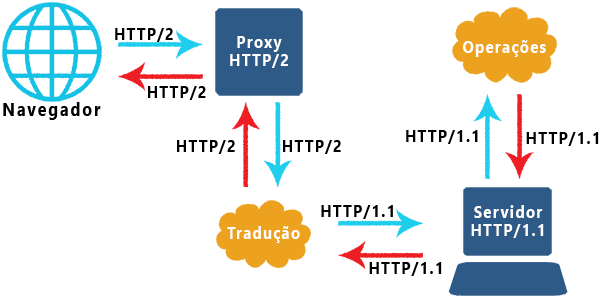
\includegraphics[width=1.0\textwidth]{./04-figuras/desenvolvimento/http2_proxy_diagram}
    \label{fig:http2diagram}
\end{figure}

Apesar de parecer muito custoso, a implementação desse \textit{proxy} já garante ao usuário uma melhora de desempenho de seu servidor, isso porque a comunicação HTTP/2 é mais rápida e melhora o paralelismos das conexões. Além disso, o \textit{proxy} ainda possibilita o uso de funcionalidades especificas do HTTP/2, como o \textit{Server Push}.

A segunda opção utiliza o \textit{nghttpd}, um servidor completo embutido dentro do \textit{nghttp2}, para fazer todo o trabalho. Dessa forma o navegador se comunica com esse servidor que faz todo o processamento necessário e retorna a resposta para o navegador. Tudo isso utilizando o protocolo HTTP/2. A desvantagem desse método é que o \textit{nghttpd} não possui um arquivo de configuração, que é uma característica típica de servidores como o Apache e o Nginx, e por isso ele acaba sendo limitado em alguns casos. Por exemplo, ainda não é possível utilizar o \textit{Server Push} com o \textit{nghttpd}, pois para configurar essa funcionalidade é necessário um arquivo de configuração.

Como os servidores de teste para cada protocolo já são diferentes, houve um grande esforço para deixar as configurações de ambiente restantes as mais similares possíveis, tentando assim evitar diferenças de desempenho provindas de outras configurações além da mudança de protocolo. Dessa forma, a escolha pela configuração utilizando o \textit{nghttpx} foi descartada. O redirecionamento via \textit{proxy} acrescentaria mais uma etapa no processo de comunicação cliente-servidor, e mesmo que se um \textit{proxy} fosse configurado para o servidor HTTP/1.1, ainda assim existe a etapa de tradução que não teria como ser simulada. Com isso, a configuração escolhida foi o uso do \textit{nghttpd}.

Como dito anteriormente, apesar de o HTTP/2 ter sido pensado inicialmente para funcionar apenas sob o protocolo TLS para melhorar a segurança da \textit{Web}, essa proposta não foi aprovada e o protocolo pode ser executado tanto com certificados de segurança como sem. Inicialmente a intenção era executar os testes nos dois ambientes, HTTP e HTTPS, contudo o \textit{nghttpd} não funcionou corretamente quando foi executado sem um certificado de segurança por isso os testes foram feitos apenas com o protocolo HTTPS. Esse tipo de falha no servidor, embora seja um problema para aplicações que querem utilizar do novo protocolo, são esperadas, pela tecnologia ser ainda muito nova e não houve tempo ábil para corrigir todos os defeitos.

\subsection{Utilizando o \textit{nghttpd}}
\label{utilizandoonghttpd}

Para utilizar o \textit{nghttpd} foi necessário uma porta possa ser escutada pelo novo servidor, um arquivo de certificado digital e uma chave para tal certificado. Então, tendo o \textit{nghttp2} instalado, basta executar o seguinte comando:

\textbf{sudo nghttpd 83 /etc/apache2/ssl/dreamtech.key /etc/apache2/ssl/dreamtech.crt -d/var/www/html/tcc -v}

\begin{itemize}
	\item 83 define qual porta será escutada pelo servidor
	\item /etc/apache2/ssl/dreamtech.key é o caminho para o arquivo de chave do certificado digital
	\item /etc/apache2/ssl/dreamtech.crt é o caminho para o certificado digital
	\item -d define que uma pasta diferente da atual será servido pelo servidor
	\item /var/www/html/tcc é o caminho da pasta que será servida
	\item -v define que o servidor deverá exibir (verbalizar) as operações que está executando
\end{itemize}

Com isso o servidor para o protocolo HTTP/2 já está funcionando, apontando para a pasta /var/www/html/tcc e já pode ser acessado pela porta 83.

\subsection{Técnicas Escolhidas}
\label{tecnicasescolhidas}

Após análise das técnicas propostas por Steve Souders em seus livros, foi concluído que cinco técnicas podem sofrer alterações com a implantação do novo protocolo. São essas:

\begin{enumerate}
	\item Faça menos requisições HTTP
	\item Reduza o número de pesquisas DNS
	\item Evite redirecionamentos
	\item Lidando com \textit{scripts} assíncronos
	\item Quebrando domínios dominantes
\end{enumerate}

Das cinco técnicas listadas acima apenas três puderão ser testadas. Isso porque para testar a técnica 3 (três) é necessário um arquivo de configurações, o que ainda não é suportado pelo \textit{nghttpd} e a funcionalidade que melhorará o desempenho da técnica 4 (quatro) ainda não foi implementada no \textit{nghttp2}.

Sendo assim apenas três técnicas propostas por Steve Souder foram testadas. Mas, para complementar a análise da melhora de desempenho causada pelo HTTP/2, um quarto teste foi feito utilizando um \textit{template} pronto e simplesmente o executando no HTTP/1.1 e depois no HTTP/2.

Para cada teste foram criados projetos HTML separados. Dessa forma o comportamento de uma técnica não interfere na outra. Além disso, foram escolhidos arquivos CSS e \textit{javascript} de maneira aleatória para a realização dos testes. Esses arquivos são de bibliotecas famosas e não foram alterados, apenas concatenados na realização de testes que necessitavam o uso dessa técnica. As bibliotecas escolhidas foram:

\begin{itemize}
	\item Animate CSS (\textit{https://daneden.github.io/animate.css/})
	\item Bootstrap (\textit{http://getbootstrap.com/})
	\item JQuery (\textit{https://jquery.com/})
	\item Font Awesome (\textit{https://fortawesome.github.io/Font-Awesome/})
	\item Full Calendar (\textit{http://fullcalendar.io/})
	\item Normalize (\textit{https://necolas.github.io/normalize.css/})
	\item Skeleton (\textit{http://getskeleton.com/})
	\item Angular JS (\textit{https://angularjs.org/})
	\item Backbone JS (\textit{http://backbonejs.org/})
	\item D3 (\textit{http://d3js.org/})
	\item Ember JS (\textit{http://emberjs.com/})
	\item High Charts (\textit{http://www.highcharts.com/})
	\item Moment JS (\textit{http://momentjs.com/})
	\item Require JS (\textit{http://requirejs.org/})
\end{itemize}

Com o intuito de estressar a conexão simulando melhor o número de requisições de um site real, nos três primeiros testes, foram inseridas na página 28 imagens de diferentes tamanhos e formatos. Essa imagens são aleatórias e nunca são alteradas.

Abaixo encontram-se a explicações de cada teste e os códigos fontes podem ser encontrados anexados ao final deste trabalho.

\subsubsection{Faça menos requisições HTTP}
\label{facamenosrequisicoeshttp}

Para a realização desse teste vários arquivos CSS e \textit{javascript} foram inseridos na página. Primeiramente os arquivos são inseridos separadamente e depois são concatenados e inseridos de uma só vez. A soma dos tamanhos dos arquivos separados é 285kB maior do que a soma dos arquivos concatenados, isso ocorre por causa da remoção de espaços em branco.

O código para o teste com arquivos separados pode ser encontrado no \autoref{apend:codigo_facamenosrequisicoeshttp_sep} e o código para o teste com os arquivos concatenados no \autoref{apend:codigo_facamenosrequisicoeshttp_concat}.

\subsubsection{Reduza o número de pesquisas DNS}
\label{reduzaonumerodepesquisasdns}

Nesse teste os mesmos arquivos CSS e \textit{javascript} do teste \ref{facamenosrequisicoeshttp} foram utilizados, mas dessa vez, ao invés de serem hospedados no mesmo servidor dos arquivos HTML, eles foram inseridos via CDN. Sendo assim a diferença está no numero de CDNs utilizadas. Enquanto no código do \autoref{apend:codigo_reduzaonumerodepesquisasdns_mult} são utilizadas 4 CNDs diferentes, no código do \autoref{apend:codigo_reduzaonumerodepesquisasdns_unic} apenas uma é utilizada. Com isso, no primeiro teste são feitas quatro consultas de DNS e no segundo apenas uma.

\subsubsection{Quebrando domínios dominantes}
\label{quebrandodominiosdominantes}

Enquanto que no teste \autoref{reduzaonumerodepesquisasdns} o número de pesquisas de DNS vai de um extremo ao outro, passa de 4 para 1, nesse teste as medições são repetidas para 2 e 3 DNS diferentes na página, com o intuito de se encontrar o número ideal de consultas de DNS que diminui o tempo de pesquisas e aumenta o paralelismo das requisições. O código para esse teste encontra-se no \autoref{apend:quebrandodominiodominantes}.

\subsection{Realização dos testes}
\label{realizacaodostestes}

Para iniciar os testes foi necessário garantir que os navegadores escolhidos estavam com a opção de realizar requisições HTTP/2 habilitada. Enquanto que nas versões mais atuais do Google Chrome está opção já vem habilitada por padrão e não existe mais uma forma de desabilita-la, no Mozilla Firefox foi necessário seguir o procedimento descrito abaixo para garantir que o navegador fizesse as requisições com o novo protocolo.

\begin{enumerate}
	\item Abre o navegador
	\item Digite \textit{about:config} na barra de navegação
	\item Confirme que deseja alterar as configurações do seu navegador
	\item Na barra de pesquisa, procure por \textit{network.http.spdy.enabled.http2draft}
	\item Clique duas vezes na preferência e confirma que seu resultado foi alterado para verdadeiro
	\item Na barra de pesquisa, procure por \textit{security.ssl.enable\_alpn}
	\item Clique duas vezes na preferência e confirma que seu resultado foi alterado para verdadeiro	
\end{enumerate}

Por fim, para garantir que os navegadores estavam fazendo requisições HTTP/2, bastou iniciar o servidor \textit{nghttpd} e utilizar as ferramentas de desenvolvedor de cada navegador.

\begin{figure}[!htb]
    \centering
    \caption{Ferramentas do desenvolvedor do Google Chrome mostrando protocolo usado na requisição.}
    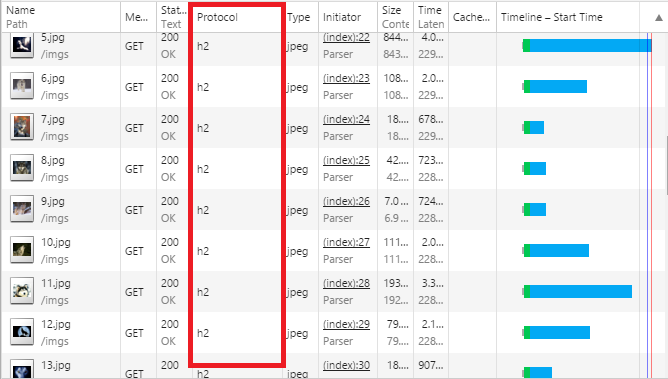
\includegraphics[width=1.0\textwidth]{./04-figuras/desenvolvimento/http2_chrome}
    \label{fig:httpcontenttype2011}
\end{figure}

\begin{figure}[!htb]
    \centering
    \caption{Ferramentas do desenvolvedor do Mozilla Firefox mostrando protocolo usado na requisição.}
    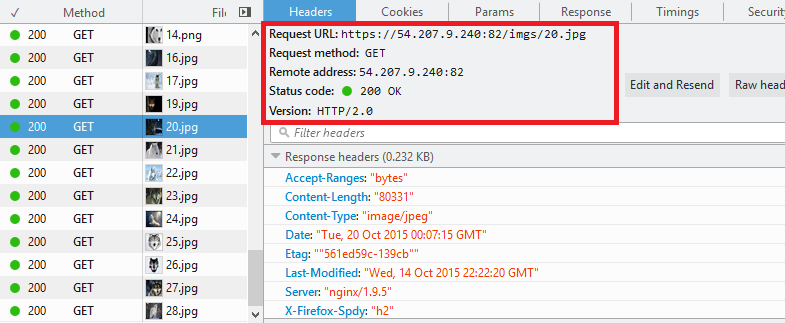
\includegraphics[width=1.0\textwidth]{./04-figuras/desenvolvimento/http2_firefox}
    \label{fig:httpcontenttype2011}
\end{figure}

Esse processo garantiu que o servidor e os navegadores funcionam, pois ambos podem se comunicar utilizando o protocolo HTTP/2. Sendo assim, pôde se dar inicio ao processo de realização dos testes.

Como o servidor \textit{nghttpd} não possui um arquivo de configuração, foi necessário colocar cada caso de teste em pastas diferentes e quando um caso novo fosse ser testado o servidor tinha de ser reiniciado e apontado para outra pasta.

Para cada técnica de otimização escolhida a página foi carregado 20 vezes utilizando o protocolo HTTP/1.1 no servidor \textit{Nginx} e 20 vezes utilizando o protocolo HTTP/2 no servidor \textit{nghttpd}. Os tempos de carregamentos das páginas foram registrado e foram calculadas as médias e medianas para cada técnica de otimização.           % Desenvolvimento
	%
% Documento: Conclusão
%

\chapter{Conclusão}
\label{chap:conclusao}

Espera-se que o uso do estilo de formatação LATEX adequado às Normas para Elaboração de Trabalhos Acadêmicos do CEFET-MG ({\ttfamily abntex2-cefetmg.cls}) facilite a escrita de documentos no âmbito desta instituição e aumente a produtividade de seus autores. Para usuários iniciantes em LATEX, além da bibliografia especializada já citada, existe ainda uma série de recursos \cite{CTAN2009} e fontes de informação \cite{TeX-Br2009,Wikibooks2009} disponíveis na Internet.

Recomenda-se o editor de textos Kile como ferramenta de composição de documentos em LATEX para usuários Linux. Para usuários Windows recomenda-se o editor TEXnicCenter \cite{TeXnicCenter2009}. O LATEX normalmente já faz parte da maioria das distribuições Linux, mas no sistema operacional Windows é necessário instalar o software MiKTeX \cite{MiKTeX2009}.

Além disso, recomenda-se o uso de um gerenciador de referências como o JabRef\index{JabRef} \cite{JabRef2009} ou Mendeley \cite{Mendeley2009} para a catalogação bibliográfica em um arquivo BIBTEX, de forma a facilitar citações através do comando \verb#\cite{}# e outros comandos correlatos do pacote ABNTEX. A lista de referências deste documento foi gerada automaticamente pelo software LATEX + BIBTEX a partir do arquivo {\ttfamily refbase.bib}, que por sua vez foi composto com o gerenciador de referências JabRef.

\section{Trabalhos futuros}
\label{sec:trabalhosFuturos}

Inserir seu texto aqui...
           % Conclusão

    % Elementos pós textuais
    \postextual
    %
% Documento: Referências Bibliográficas
%

\bibliography{./refbase}    % Geração automática das referências por meio do arquivo 'refbase.bib'
       % Referências
    %
% Documento: Apêndices
%

\begin{apendicesenv}
\partapendices

\chapter{Tentativa de configuração do mod\_h2}
\label{apend:tentativadeconfiguracaomodh2}

Na tentativa de configurar o módulo moh\_h2 em um servidor Apache, foram usadas como referência as instruções descritas no site do projeto\footnote{https://github.com/icing/mod\_h2} no mês de Agosto de 2015. Mas apesar das instruções estarem bem explicadas, o final do processo de configuração ficou um pouco confuso e com isso não foi possível concluir a instalação do mod\_h2 com sucesso.

Abaixo encontra-se o passo-a-passo realizado.

\begin{enumerate}
	\item Clone o projeto para conseguir o código: \textit{git clone https://github.com/icing/mod\_h2.git}
	\item Instale as dependências de sistema necessárias: \textit{sudo apt-get install git gcc g++ libpcre3-dev libcunit1-dev libev-dev libjansson-dev libjemalloc-dev cython make binutils autoconf automake autotools-dev libtool pkg-config zlib1g-dev libssl-dev libxml2-dev libevent-dev python3.4-dev libevent-openssl-2.0-5 php5-cgi python-setuptools}
	\item Entre na pasta do projeto: \textit{cd mod\_h2-x.x.x}
	\item Gere os arquivos necessários para o automake e o autoconf funcionarem: \textit{autoreconf -i}
	\item Gere o arquivo de compilação: \textit{automake}
	\item Gere o arquivo de configuração: \textit{autoconf}
	\item Execute o \textit{script} de configuração: \textit{./configure --enable-sandbox}\footnote{A instalação utilizando a \textit{sandbox} garante que todas as dependências para configurar o servidor serão instaladas.}
	\item Compile o código: \textit{make}
	\item Encontre o arquivo binário (mod\_h2.so) gerado
	\item Crie ma pasta chamada \textit{modules} e copie o arquivo binário para ela
	\item Mude a configuração geral do servidor Apache para utilizar o novo módulo:
		\begin{center}
			\textit{sudo nano apache2.conf}
			Adicione o seguinte código na última linha do arquivo: \textit{LoadModule h2\_module /etc/apache2/modules/mod\_h2.so} (onde /etc/apache2/modules/mod\_h2.so é o caminho para seu arquivo binário)
		\end{center}
	\item Reinicie o servidor: \textit{sudo service apache2 restart}
\end{enumerate}

Juntamente com as configurações de navegador necessárias para garantir que as requisições serão feitas utilizando o novo protocolo, essa sequencia de passos deveria ser o suficiente para garantir que o servidor Apache iria utilizar o protocolo HTTP/2. Mas apesar de nenhum erro ter ocorrido durante o processo, a comunicação dos dado não passou a ser realizada com o HTTP/2.

Como o mod\_h2 é um projeto que está em desenvolvimento, muitas atualizações são feitas toda semana e a documentação sempre está evoluindo. Sendo assim pode se esperar que a documentação esteja mais completa na data de publicação deste trabalho e que a configuração do módulo seja mais fácil.

Ademais, vale ressaltar que o mod\_h2 foi doado à Apache Foundation e que ele se tornará o módulo oficial para o HTTP/2 do servidor Apache na sua versão 2.4. O lançamento da nova versão do servidor está prevista para Outubro de 2015.

\chapter{Configurando \textit{nghttp2}}
\label{apend:configurandonghttp2}

Apesar de descrita no site oficial do projeto\footnote{https://github.com/tatsuhiro-t/nghttp2}, a configuração do \textit{nghttp2} só foi possível graças a \citeonline{nghttp2config}. Em seu artigo Tollman descreve bem detalhadamente o processo de instalação do \textit{nghttp2} e suas dependências. Enquanto que no site oficial do projeto a instalação das dependências fica a cargo do desenvolvedor. 

Abaixo encontra-se um resumo dos passos descritos por Tollman.

\subsection{Instalando dependências}
Instale todas as dependências básicas:
	\begin{center}
		\textit{sudo apt-get install make binutils autoconf automake autotools-dev libtool pkg-config zlib1g-dev libcunit1-dev libssl-dev libxml2-dev libev-dev libevent-dev libjansson-dev libjemalloc-dev python3.4-dev g++ g++-mingw-w64-i686 git python3-setuptools}	
		\textit{sudo easy\_install3 pip}
		\textit{sudo pip3.4 install -U cython}
	\end{center}

Instale o Spdylay, que serve como base para o \textit{nghttp2}
\begin{enumerate}
	\item Crie uma pasta para o código compilado: \textit{mkdir ~/src}
	\item Clone o projeto: \textit{git clone https://github.com/tatsuhiro-t/spdylay.git ~/src/spdylay}
	\item Entre na pasta: \textit{cd ~/src/spdylay}
	\item Gere os arquivos necessários para o automake e o autoconf funcionarem: \textit{autoreconf -i}
	\item Gere o arquivo de compilação: \textit{automake}
	\item Gere o arquivo de configuração: \textit{autoconf}
	\item Execute o \textit{script} de configuração: \textit{./configure}
	\item Compile o código: \textit{make}
	\item Execute o arquivo compilado: \textit{sudo make install}
	\item Atualize o seu sistema: \textit{sudo updatedb}
	\item Localize a biblioteca spylay: \textit{locate libspdylay.so.7}
	\item Configure os links de execução da biblioteca:
		\begin{center}
			\textit{sudo ln -s /usr/local/lib/libspdylay.so.7 /lib/x86\_64-linux-gnu/libspdylay.so.7}
			\textit{sudo ln -s /usr/local/lib/libspdylay.so.7.2.0 /lib/x86\_64-linux-gnu/libspdylay.so.7.2.0}
			\textit{sudo ldconfig}
		\end{center}
\end{enumerate}

Seguindo esses passos todas dependências necessárias para a instalação do \textit{nghttps} estão prontas para serem usadas.

\subsection{Instalando a aplicação}
O processo de instalação do \textit{nghttp2} é mais uma vez um processo de compilação do código fonte e configuração da biblioteca.

\begin{enumerate}
	\item Clone o projeto: \textit{git clone https://github.com/tatsuhiro-t/nghttp2.git ~/src/nghttp2}
	\item Entre na pasta: \textit{cd ~/src/nghttp2}
	\item Gere os arquivos necessários para o automake e o autoconf funcionarem: \textit{autoreconf -i}
	\item Gere o arquivo de compilação: \textit{automake}
	\item Gere o arquivo de configuração: \textit{autoconf}
	\item Execute o \textit{script} de configuração: \textit{./configure PYTHON=/usr/bin/python3} (confirmar o uso do \textit{python3} é muito importante, pois por padrão o \textit{python2} que costuma ser utilizado)
	\item Compile o código: \textit{make}
	\item Execute o arquivo compilado: \textit{sudo make install}
	\item Atualize o seu sistema: \textit{sudo updatedb}
	\item Localize a biblioteca spylay: \textit{locate libnghttp2.so.14}
	\item Configure os links de execução da biblioteca:
		\begin{center}
			\textit{sudo ln -s /usr/local/lib/libnghttp2.so.14 /lib/x86\_64-linux-gnu/libnghttp2.so.14}
			\textit{sudo ln -s /usr/local/lib/libnghttp2.so.14.0.2 /lib/x86\_64-linux-gnu/libnghttp2.so.14.0.2}
			\textit{sudo ldconfig}
		\end{center}
\end{enumerate}

Vale ressaltar que as versões especificadas nos arquivos gerados dependem das versões dos códigos que estão sendo utilizados.

\lstset{
	frame=single,
    breaklines=true,
    language=HTML
    }
\chapter{Faça menos requisições HTTP: Arquivos Separados}
\label{apend:codigo_facamenosrequisicoeshttp_sep}

\begin{lstlisting}
<!DOCTYPE html>
<html>
<head>
<link rel="stylesheet" href="css/animate.css">
<link rel="stylesheet" href="css/bootstrap.min.css">
<link rel="stylesheet" href="css/bootstrap-theme.min.css">
<link rel="stylesheet" href="css/font-awesome.min.css">
<link rel="stylesheet" href="css/fullcalendar.min.css">
<link rel="stylesheet" href="css/normalize.css">
<link rel="stylesheet" href="css/skeleton.css">
	
<link rel="stylesheet" href="css/animate - Copy.css">
<link rel="stylesheet" href="css/bootstrap.min - Copy.css">
<link rel="stylesheet" href="css/bootstrap-theme.min - Copy.css">
<link rel="stylesheet" href="css/font-awesome.min - Copy.css">
<link rel="stylesheet" href="css/fullcalendar.min - Copy.css">
<link rel="stylesheet" href="css/normalize - Copy.css">
<link rel="stylesheet" href="css/skeleton - Copy.css">
</head>

<body>

<h1>My First Heading</h1>

<p>My first paragraph.</p>

<img src="imgs/1.jpg" />
<img src="imgs/2.jpg" />
<img src="imgs/3.jpg" />
<img src="imgs/4.jpg" />
<img src="imgs/5.jpg" />
<img src="imgs/6.jpg" />
<img src="imgs/7.jpg" />
<img src="imgs/8.jpg" />
<img src="imgs/9.jpg" />
<img src="imgs/10.jpg" />
<img src="imgs/11.jpg" />
<img src="imgs/12.jpg" />
<img src="imgs/13.jpg" />
<img src="imgs/14.png" />
<img src="imgs/15.png" />
<img src="imgs/16.jpg" />
<img src="imgs/17.jpg" />
<img src="imgs/18.jpg" />
<img src="imgs/19.jpg" />
<img src="imgs/20.jpg" />
<img src="imgs/21.jpg" />
<img src="imgs/22.jpg" />
<img src="imgs/23.jpg" />
<img src="imgs/24.jpg" />
<img src="imgs/25.jpg" />
<img src="imgs/26.jpg" />
<img src="imgs/27.jpg" />
<img src="imgs/28.jpg" />
	

<script src="js/jquery-2.1.4.min.js"></script>
<script src="js/angular.min.js"></script>
<script src="js/backbone.js"></script>
<script src="js/bootstrap.min.js"></script>
<script src="js/d3.min.js"></script>
<script src="js/ember-data.min.js"></script>
<script src="js/fullcalendar.min.js"></script>
<script src="js/highcharts.js"></script>
<script src="js/moment-with-locales.min.js"></script>
<script src="js/require.js"></script>
</body>
</html>
\end{lstlisting}

\chapter{Faça menos requisições HTTP: Arquivos Concatenados}
\label{apend:codigo_facamenosrequisicoeshttp_concat}

\begin{lstlisting}
<!DOCTYPE html>
<html>
<head>
<link rel="stylesheet" href="css/minified.css">
</head>

<body>

<h1>My First Heading</h1>
<p>My first paragraph.</p>
	
<img src="imgs/1.jpg" />
<img src="imgs/2.jpg" />
<img src="imgs/3.jpg" />
<img src="imgs/4.jpg" />
<img src="imgs/5.jpg" />
<img src="imgs/6.jpg" />
<img src="imgs/7.jpg" />
<img src="imgs/8.jpg" />
<img src="imgs/9.jpg" />
<img src="imgs/10.jpg" />
<img src="imgs/11.jpg" />
<img src="imgs/12.jpg" />
<img src="imgs/13.jpg" />
<img src="imgs/14.png" />
<img src="imgs/15.png" />
<img src="imgs/16.jpg" />
<img src="imgs/17.jpg" />
<img src="imgs/18.jpg" />
<img src="imgs/19.jpg" />
<img src="imgs/20.jpg" />
<img src="imgs/21.jpg" />
<img src="imgs/22.jpg" />
<img src="imgs/23.jpg" />
<img src="imgs/24.jpg" />
<img src="imgs/25.jpg" />
<img src="imgs/26.jpg" />
<img src="imgs/27.jpg" />
<img src="imgs/28.jpg" />

	<script src="js/minified.js"></script>
</body>
</html>

\end{lstlisting}

\chapter{Reduza o número de pesquisas DNS: Multiplas CDN}
\label{apend:codigo_reduzaonumerodepesquisasdns_mult}	

\begin{lstlisting}
<!DOCTYPE html>
<html>
<head>
<link rel="stylesheet" href="//cdnjs.cloudflare.com/ajax/libs/animate.css/3.4.0/animate.min.css">
<link rel="stylesheet" href="//maxcdn.bootstrapcdn.com/bootstrap/3.3.5/css/bootstrap.min.css">
<link rel="stylesheet" href="//maxcdn.bootstrapcdn.com/font-awesome/4.4.0/css/font-awesome.min.css">	
<link rel="stylesheet" href="//cdnjs.cloudflare.com/ajax/libs/fullcalendar/2.0.2/fullcalendar.js">
<link rel="stylesheet" href="//cdn.bootcss.com/skeleton/2.0.4/skeleton.css">
<link rel="stylesheet" href="css/normalize.css">
</head>

<body>

<h1>My First Heading</h1>
<p>My first paragraph.</p>

<img src="imgs/1.jpg" />
<img src="imgs/2.jpg" />
<img src="imgs/3.jpg" />
<img src="imgs/4.jpg" />
<img src="imgs/5.jpg" />
<img src="imgs/6.jpg" />
<img src="imgs/7.jpg" />
<img src="imgs/8.jpg" />
<img src="imgs/9.jpg" />
<img src="imgs/10.jpg" />
<img src="imgs/11.jpg" />
<img src="imgs/12.jpg" />
<img src="imgs/13.jpg" />
<img src="imgs/14.png" />
<img src="imgs/15.png" />
<img src="imgs/16.jpg" />
<img src="imgs/17.jpg" />
<img src="imgs/18.jpg" />
<img src="imgs/19.jpg" />
<img src="imgs/20.jpg" />
<img src="imgs/21.jpg" />
<img src="imgs/22.jpg" />
<img src="imgs/23.jpg" />
<img src="imgs/24.jpg" />
<img src="imgs/25.jpg" />
<img src="imgs/26.jpg" />
<img src="imgs/27.jpg" />
<img src="imgs/28.jpg" />

<script src="//ajax.googleapis.com/ajax/libs/jquery/2.1.4/jquery.min.js"></script>
<script src="//maxcdn.bootstrapcdn.com/bootstrap/3.3.5/js/bootstrap.min.js"></script>
<script src="//ajax.googleapis.com/ajax/libs/angularjs/1.3.14/angular.min.js"></script>
<script src="//cdnjs.cloudflare.com/ajax/libs/d3/3.5.6/d3.js"></script>
<script src="//cdn.bootcss.com/ember.js/2.1.0-beta.2/ember.js"></script>
<script src="js/require.js"></script>	
</body>
</html>

\end{lstlisting}

\chapter{Reduza o número de pesquisas DNS: Única CDN}
\label{apend:codigo_reduzaonumerodepesquisasdns_unic}	

\begin{lstlisting}
<!DOCTYPE html>
<html>
<head>
<link rel="stylesheet" href="//cdnjs.cloudflare.com/ajax/libs/animate.css/3.4.0/animate.min.css">
<link rel="stylesheet" href="//cdnjs.cloudflare.com/ajax/libs/twitter-bootstrap/4.0.0-alpha/js/bootstrap.min.js">
<link rel="stylesheet" href="//cdnjs.cloudflare.com/ajax/libs/font-awesome/4.4.0/css/font-awesome.min.css">	
<link rel="stylesheet" href="//cdnjs.cloudflare.com/ajax/libs/fullcalendar/2.0.2/fullcalendar.js">
<link rel="stylesheet" href="//cdnjs.cloudflare.com/ajax/libs/skeleton/2.0.4/skeleton.css">
<link rel="stylesheet" href="//cdnjs.cloudflare.com/ajax/libs/normalize/3.0.3/normalize.css">
</head>

<body>

<h1>My First Heading</h1>
<p>My first paragraph.</p>

<img src="imgs/1.jpg" />
<img src="imgs/2.jpg" />
<img src="imgs/3.jpg" />
<img src="imgs/4.jpg" />
<img src="imgs/5.jpg" />
<img src="imgs/6.jpg" />
<img src="imgs/7.jpg" />
<img src="imgs/8.jpg" />
<img src="imgs/9.jpg" />
<img src="imgs/10.jpg" />
<img src="imgs/11.jpg" />
<img src="imgs/12.jpg" />
<img src="imgs/13.jpg" />
<img src="imgs/14.png" />
<img src="imgs/15.png" />
<img src="imgs/16.jpg" />
<img src="imgs/17.jpg" />
<img src="imgs/18.jpg" />
<img src="imgs/19.jpg" />
<img src="imgs/20.jpg" />
<img src="imgs/21.jpg" />
<img src="imgs/22.jpg" />
<img src="imgs/23.jpg" />
<img src="imgs/24.jpg" />
<img src="imgs/25.jpg" />
<img src="imgs/26.jpg" />
<img src="imgs/27.jpg" />
<img src="imgs/28.jpg" />

<script src="//cdnjs.cloudflare.com/ajax/libs/jquery/2.1.4/jquery.min.js"></script>
<script src="//cdnjs.cloudflare.com/ajax/libs/twitter-bootstrap/3.3.5/js/bootstrap.min.js"></script>
<script src="//cdnjs.cloudflare.com/ajax/libs/angular.js/1.3.14/angular.min.js"></script>
<script src="//cdnjs.cloudflare.com/ajax/libs/d3/3.5.6/d3.js"></script>
<script src="//cdnjs.cloudflare.com/ajax/libs/ember.js/2.1.0-beta.2/ember.js"></script>
<script src="//cdnjs.cloudflare.com/ajax/libs/require.js/2.1.20/require.min.js"></script>	
</body>
</html>

\end{lstlisting}

\chapter{Quebrando domínios dominantes}
\label{apend:quebrandodominiodominantes}

Para duas CDNs
\begin{lstlisting}
<!DOCTYPE html>
<html>
<head>
<link rel="stylesheet" href="//cdnjs.cloudflare.com/ajax/libs/animate.css/3.4.0/animate.min.css">
<link rel="stylesheet" href="//maxcdn.bootstrapcdn.com/bootstrap/3.3.5/css/bootstrap.min.css">
<link rel="stylesheet" href="//maxcdn.bootstrapcdn.com/font-awesome/4.4.0/css/font-awesome.min.css">	
<link rel="stylesheet" href="//cdnjs.cloudflare.com/ajax/libs/fullcalendar/2.0.2/fullcalendar.js">
<link rel="stylesheet" href="//cdnjs.cloudflare.com/ajax/libs/skeleton/2.0.4/skeleton.css">
<link rel="stylesheet" href="//cdnjs.cloudflare.com/ajax/libs/normalize/3.0.2/normalize.css">
</head>

<body>

<h1>My First Heading</h1>
<p>My first paragraph.</p>
	
<img src="imgs/1.jpg" />
<img src="imgs/2.jpg" />
<img src="imgs/3.jpg" />
<img src="imgs/4.jpg" />
<img src="imgs/5.jpg" />
<img src="imgs/6.jpg" />
<img src="imgs/7.jpg" />
<img src="imgs/8.jpg" />
<img src="imgs/9.jpg" />
<img src="imgs/10.jpg" />
<img src="imgs/11.jpg" />
<img src="imgs/12.jpg" />
<img src="imgs/13.jpg" />
<img src="imgs/14.png" />
<img src="imgs/15.png" />
<img src="imgs/16.jpg" />
<img src="imgs/17.jpg" />
<img src="imgs/18.jpg" />
<img src="imgs/19.jpg" />
<img src="imgs/20.jpg" />
<img src="imgs/21.jpg" />
<img src="imgs/22.jpg" />
<img src="imgs/23.jpg" />
<img src="imgs/24.jpg" />
<img src="imgs/25.jpg" />
<img src="imgs/26.jpg" />
<img src="imgs/27.jpg" />
<img src="imgs/28.jpg" />

<script src="//cdnjs.cloudflare.com/ajax/libs/jquery/2.1.4/jquery.min.js"></script>
<script src="//maxcdn.bootstrapcdn.com/bootstrap/3.3.5/js/bootstrap.min.js"></script>
<script src="//cdnjs.cloudflare.com/ajax/libs/angular.js/1.3.14/angular.min.js"></script>
<script src="//cdnjs.cloudflare.com/ajax/libs/d3/3.5.6/d3.js"></script>
<script src="//cdnjs.cloudflare.com/ajax/libs/ember.js/2.1.0-beta.2/ember.js"></script>
<script src="//cdnjs.cloudflare.com/ajax/libs/require.js/2.1.20/require.min.js"></script>	
</body>
</html>
\end{lstlisting}

Para três CDNs
\begin{lstlisting}
<!DOCTYPE html>
<html>
<head>
<link rel="stylesheet" href="//cdnjs.cloudflare.com/ajax/libs/animate.css/3.4.0/animate.min.css">
<link rel="stylesheet" href="//maxcdn.bootstrapcdn.com/bootstrap/3.3.5/css/bootstrap.min.css">
<link rel="stylesheet" href="//maxcdn.bootstrapcdn.com/font-awesome/4.4.0/css/font-awesome.min.css">	
<link rel="stylesheet" href="//cdnjs.cloudflare.com/ajax/libs/fullcalendar/2.0.2/fullcalendar.js">
<link rel="stylesheet" href="//cdn.bootcss.com/skeleton/2.0.4/skeleton.css">
<link rel="stylesheet" href="//cdnjs.cloudflare.com/ajax/libs/normalize/3.0.2/normalize.css">
</head>

<body>

<h1>My First Heading</h1>
<p>My first paragraph.</p>
	
<img src="imgs/1.jpg" />
<img src="imgs/2.jpg" />
<img src="imgs/3.jpg" />
<img src="imgs/4.jpg" />
<img src="imgs/5.jpg" />
<img src="imgs/6.jpg" />
<img src="imgs/7.jpg" />
<img src="imgs/8.jpg" />
<img src="imgs/9.jpg" />
<img src="imgs/10.jpg" />
<img src="imgs/11.jpg" />
<img src="imgs/12.jpg" />
<img src="imgs/13.jpg" />
<img src="imgs/14.png" />
<img src="imgs/15.png" />
<img src="imgs/16.jpg" />
<img src="imgs/17.jpg" />
<img src="imgs/18.jpg" />
<img src="imgs/19.jpg" />
<img src="imgs/20.jpg" />
<img src="imgs/21.jpg" />
<img src="imgs/22.jpg" />
<img src="imgs/23.jpg" />
<img src="imgs/24.jpg" />
<img src="imgs/25.jpg" />
<img src="imgs/26.jpg" />
<img src="imgs/27.jpg" />
<img src="imgs/28.jpg" />

<script src="//cdn.bootcss.com/jquery/2.1.4/jquery.min.js"></script>
<script src="//maxcdn.bootstrapcdn.com/bootstrap/3.3.5/js/bootstrap.min.js"></script>
<script src="//cdn.bootcss.com/angular.js/1.3.4/angular.min.js"></script>
<script src="//cdnjs.cloudflare.com/ajax/libs/d3/3.5.6/d3.js"></script>
<script src="//cdn.bootcss.com/ember.js/2.1.0-beta.2/ember.js"></script>
<script src="//cdn.bootcss.com/require.js/2.1.20/require.min.js"></script>	
</body>
</html>

\end{lstlisting}

\end{apendicesenv}
         % Apêndices
    %%
% Documento: Anexos
%

\begin{anexosenv}
\partanexos

\chapter{Nome do Anexo}
\label{chap:anexox}

Inserir seu texto aqui...

\chapter{Nome do Anexo}
\label{chap:anexoy}

Inserir seu texto aqui...

\end{anexosenv}
            % Anexos
    \printindex                                             % Índice remissivo

\end{document}
